\documentclass{article}
\usepackage{graphicx} % Required for 
\usepackage{natbib} % For bibliography
\usepackage{float} % Add this in your preamble


\title{paper collagen}
\author{robert.tavares}
\date{November 2023}

\begin{document}

\maketitle

\section{Introduction}

O colágeno tipo I é uma proteína abundante no corpo humano, de forma que compõe $90\%$ dele. Ele está presente na matriz extracelular bem como em estruturas como pele, osso, tendão e córnea \cite{RicoLlanos2021, Silver2018}.
\\

O colágeno tipo I é uma molécula composta por um tripla hélice de cadeias polipeptídicas(cadeias $\alpha$). Ele possui tamanhos típicos de $300$ nm de comprimento por $1,5$ nm de diâmetro e apresenta um formato tipo haste \cite{Gelse2003,Silver2018}. 
\\

As moléculas de colágeno tipo I possuem, intrisicamente, a informação necessária para se auto-organizar em estruturas mais complexas chamadas fibrilas. Esse processo, denominado fibrilo-gênese, ocorre o mediante a agregação de milhares dessas moléculas de forma escalonada por um período $D= 67$ nm, de modo que existem cinco posições possíveis para que ocorra a interação entre elas\cite{Zhu2018, KADLER1996}.  
\\

As fibrilas apresentam um formato alongado, com a sua região mais densa sendo a central e, consequentemente, as pontas afinadas\cite{Charvolin2019, KADLER1996}. As fibrilas apresentam comprimento típicos de $500 \mu m$ com $500 nm$ de diâmetro, além de serem constituídas por moléculas da ordem de $10^{7}$\cite{Parry1984}. 
\\


\section{Metodologia}


Em nosso trabalho, nos tivemos duas etapas desenvolvidas: Modelo para formação de fibrilas e Morfologia e propriedades mecânicas das fibrilas. 

\subsection{Formação de fibrilas}

Nos utilizamos um modelo baseado em DLA(difusion limited aggregation)\cite{Witten1983} em três dimensões para tentar simular a formação das fibrilas de colágeno. As moléculas são lançadas de uma distância $R$ da origem do nosso agregado e se difundem até encontrarem o mesmo ou atingirem uma distância  $2R$, de modo que a simulação é reiniciada caso isso ocorra. Ao atingir o agregado, a molécula é capturada apenas se ela estiver em uma posição que é um múltiplo de $D = 4$ com relação a uma molécula pertencente ao agregado\cite{Parkinson1995}. 
\\

Cada molécula é representada por um bastão de dimensão 1 x 18 x 1 e pode se mover entre os primeiros e segundos vizinhos no plano XZ, enquanto pode se mover para frente e para trás no eixo Y.
\\


O processo de formação das fibrilas é dirigido por uma força hidrofóbica devido a interação entre as moléculas, de modo que elas tentam minimizar sua superfície exposta para tal\cite{Kadler1987, Parkinson1995}. Para representar esse processo, utilizamos um algoritmo de rolamento sobre a superfície, que permite um bastão recém agregado explorar a superfície do agregado, mantendo seu y fixo, para encontrar um local que minimize sua superfície exposta\cite{GarcaRuiz1991}. Caso ocorra mais de um local, a primeira posição é mantida. Esse movimento é controlado pelo parâmetro $T_{s}$ que define o número de passos que a molécula tem para explorar a superfície do agregado\cite{Parkinson1995}.
\\

Com esse algorítimo, geramos $10$ fibrilas contendo $30.000$ bastões para diferentes valores de $T_{s}$ a fim de ver o efeito desse parâmetro na morfologia das fibrilas. 


\subsection{Propriedades das fibrilas}

Para analisar as propriedades mecânicas das fibrilas, utilizamos um modelo mecânico probabilístico, visto que as fibrilas geradas não possuem um carácter elástico para ser estudado como normalmente é feito\cite{Parkinson1997}. 

Para cada  amostra de um dado valor do parâmetro $T_{s}$, fizemos o corte de um tronco de dimensão 101 x 201 x 101 na região central das fibrilas afim de minimizar efeitos de borda. Depois, realizamos uma limpeza nesse tronco para eliminar moléculas que não estavam pertencentes ao esqueleto ativo\cite{Parkinson1997}.

Ao aplicarmos uma força no esqueleto, calculamos a pressão $\sigma$, onde a área é dada pelo número de elementos do esqueleto ativo em uma dada camada do tronco. No modelo mecânico estocástico, para cada molécula no agregado, determinamos uma probabilidade de remoção dada por:

\begin{equation}
    P_{R} = (\frac{<\sigma>}{N\sigma_{s}})^{m},
\end{equation}

\noindent onde $\sigma$ é a média da pressão que cada pedaço de uma molécula sente, $N$ é o número de ligações que uma dada molécula possui, assumimos que cada face em contato com uma molécula vizinha contribui com uma ligação, $\sigma_{c}$ a força da ligação entre as moléculas, que tomamos como unitária e m é um fator de amortecimento da energia\cite{Parkinson1997,2013}.

A simulação consiste em aplicarmos umas força no esqueleto ativo, com isso, calculamos as probabilidades de cada molécula ser removida e sortíamos um número para ver se ocorre a ruptura. Caso ocorra pelo menos uma única quebra, repetimos o procedimento para uma dada força até que não mais ocorra rupturas. Nesse ponto, incrementamos a força em meio e repetimos a simulação. A fibrila se quebra se ocorrer a existência de pelo menos uma camada vazia.

(fazer uma figura disso)

Com isso, realizamos, para cada fibrila com um determinado valor de $T_{s}$, mil experimentos. Guardamos informações dos valores, para cada força, do número removido do esqueleto, bem quantas restaram.

\section{Resultados}

\subsection{Morfologia das fibrilas}

Os agregados gerados pelo modelo apresentam uma morfologia fibrilar, com característica relevantes da sua forma sendo determinadas pelo parâmetro $T_{s}$. Nos podemos observar, na figura \ref{R1}, a forma desses agregados para os valores de $T_{s} = 2$ e $T_{s} = 10000$. As fibrilas com menor $T_{s}$ apresentam uma estrutura mais aberta, enquanto para valores mais altos, observamos uma forma mais compacta e regular. A coloração indica o quão antigo uma molécula é no agregado, indo do azul escuro, mais antigas,para o amarelo, mais recentes. Nos agregados mais compactos, temos dificuldade em observar moléculas mais antigas visto que essas estão muito dentro da estrutura. Para as mais abertas, temos uma maior facilidade em observar moléculas mais antigas. Além disso, na visão lateral, observamos o comportamento alongado e com pontas afinadas, típico de fibrilas reais. 

O comprimento e o diâmetro médio das fibrilas são características determinadas pelo parâmetro $T_{s}$. Na Tabela 1, podemos ver como essas medidas variaram, em média, com o aumento desse parâmetro. Podemos observar como, a partir de $T_{s} = 512$, as medidas parecem atingir um limite superior. 

Outra características desses agregados é a relação linear da massa em função das distâncias as pontas. Na figura \ref{R2}, temos que, independente do parâmetro $T_{s}$, todos os agregados apresentam esse comportamento.Essas características serviram de validação para o nosso modelo, visto que são observações recorrentes em fibrilas reais \cite{}.

\begin{figure}[H]
    \centering
    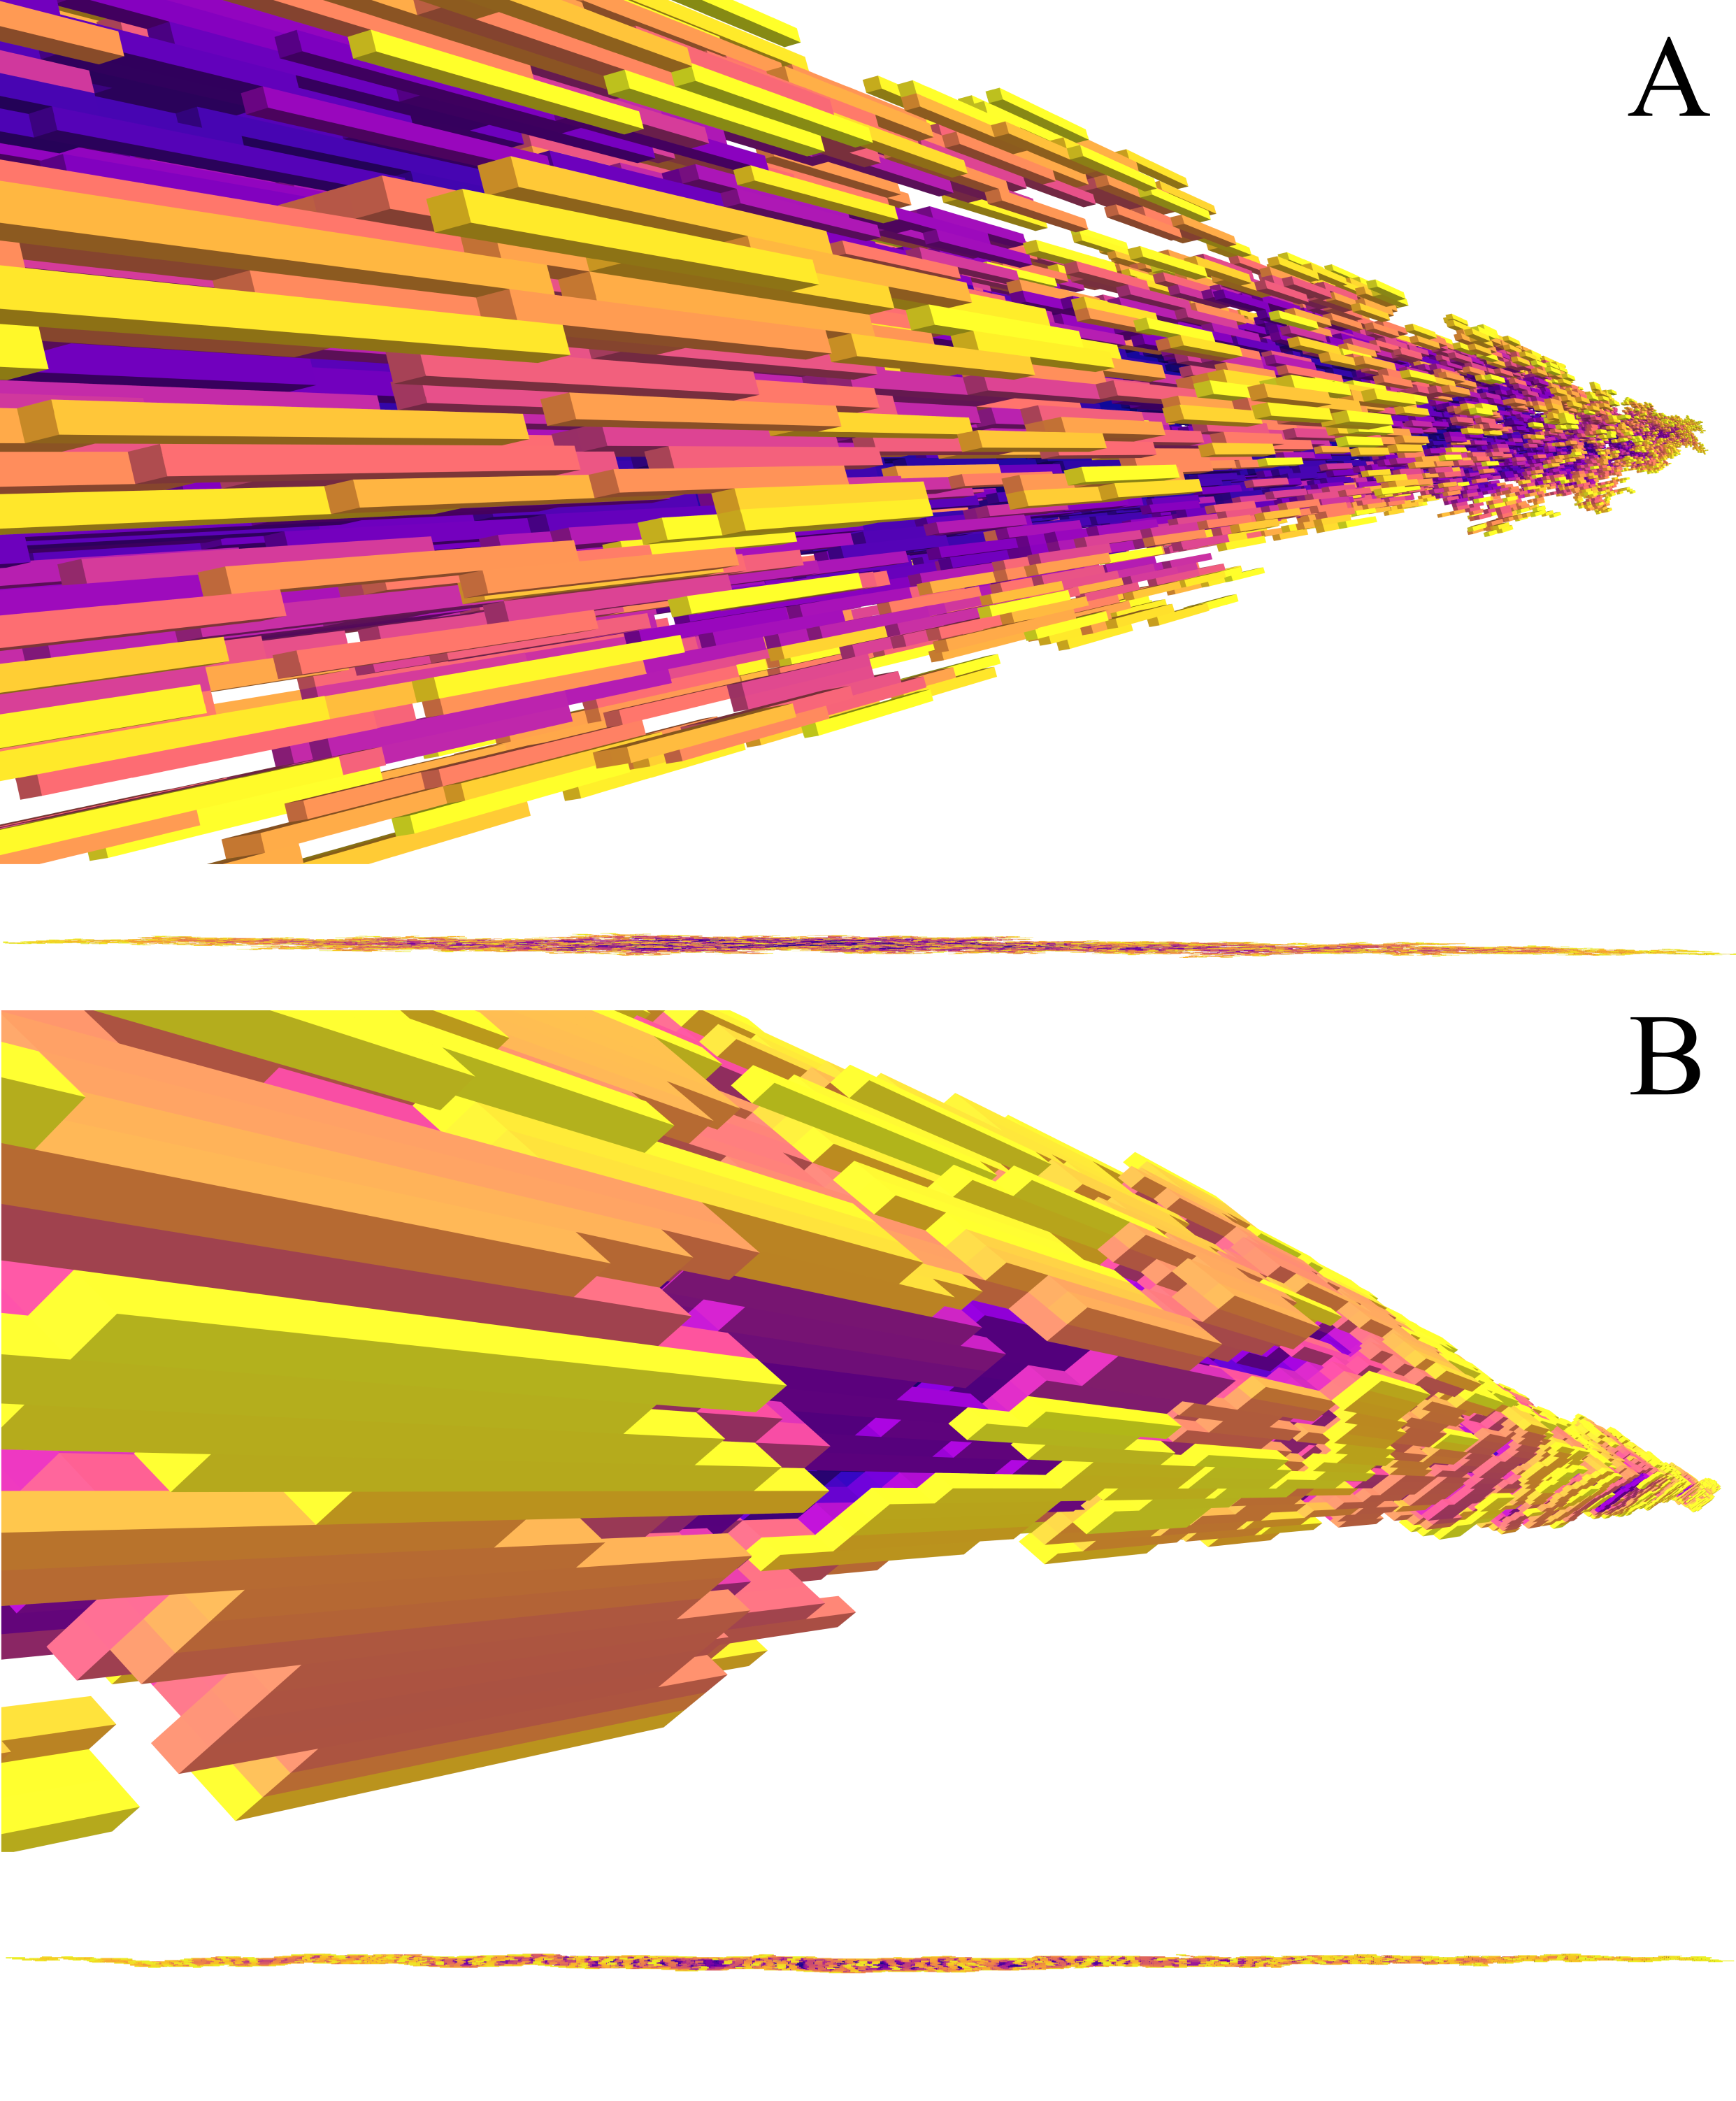
\includegraphics[width=\textwidth]{figures/fibrils.png}

    \caption{Visualização transversal e lateral das fibrilas geradas com o algoritmo de DLA. A coloração indica quão antigo é a molécula no agregado. Quanto mais pro azul escuro, mais antigo no agregado, quanto mais para o amarelo, mais recente. A) Fibrilas geradas para $T_{s} = $ 2. B) Fibrilas geradas para $T_{s} = $ 10000. } 

    \label{R1}
\end{figure}


Analizando a seção transversal das fibrilas, na Figura \ref{R3}, observamos que, o aumento do parâmetro $T_{s}$ levava a diminuição dos espaços vazios dentro da seção e formação de agregados compactos e quase totalmente preenchidos. Devido a essa característica pregressiva com o parâmetro, nos calculamos a dimensão fractal das seções e observamos que, a medida que $T_{s}$ cresce, ocorre um aumento do valor médio da dimensão fractal da seção até uma saturação. Na Figura \ref{R4}, podemos ver que para valores mais baixos, a dimensionalidade é próxima da observada em agregados gerados por DLA, 1.71, o que remete ao nosso modelo de formação, enquanto que para valores mais altos, o comportamento tende a estabilizar em valores próximos a 1.93, muito próximo da dimensão euclidiana para objetos 2D.

\begin{figure}[H]
    \centering
    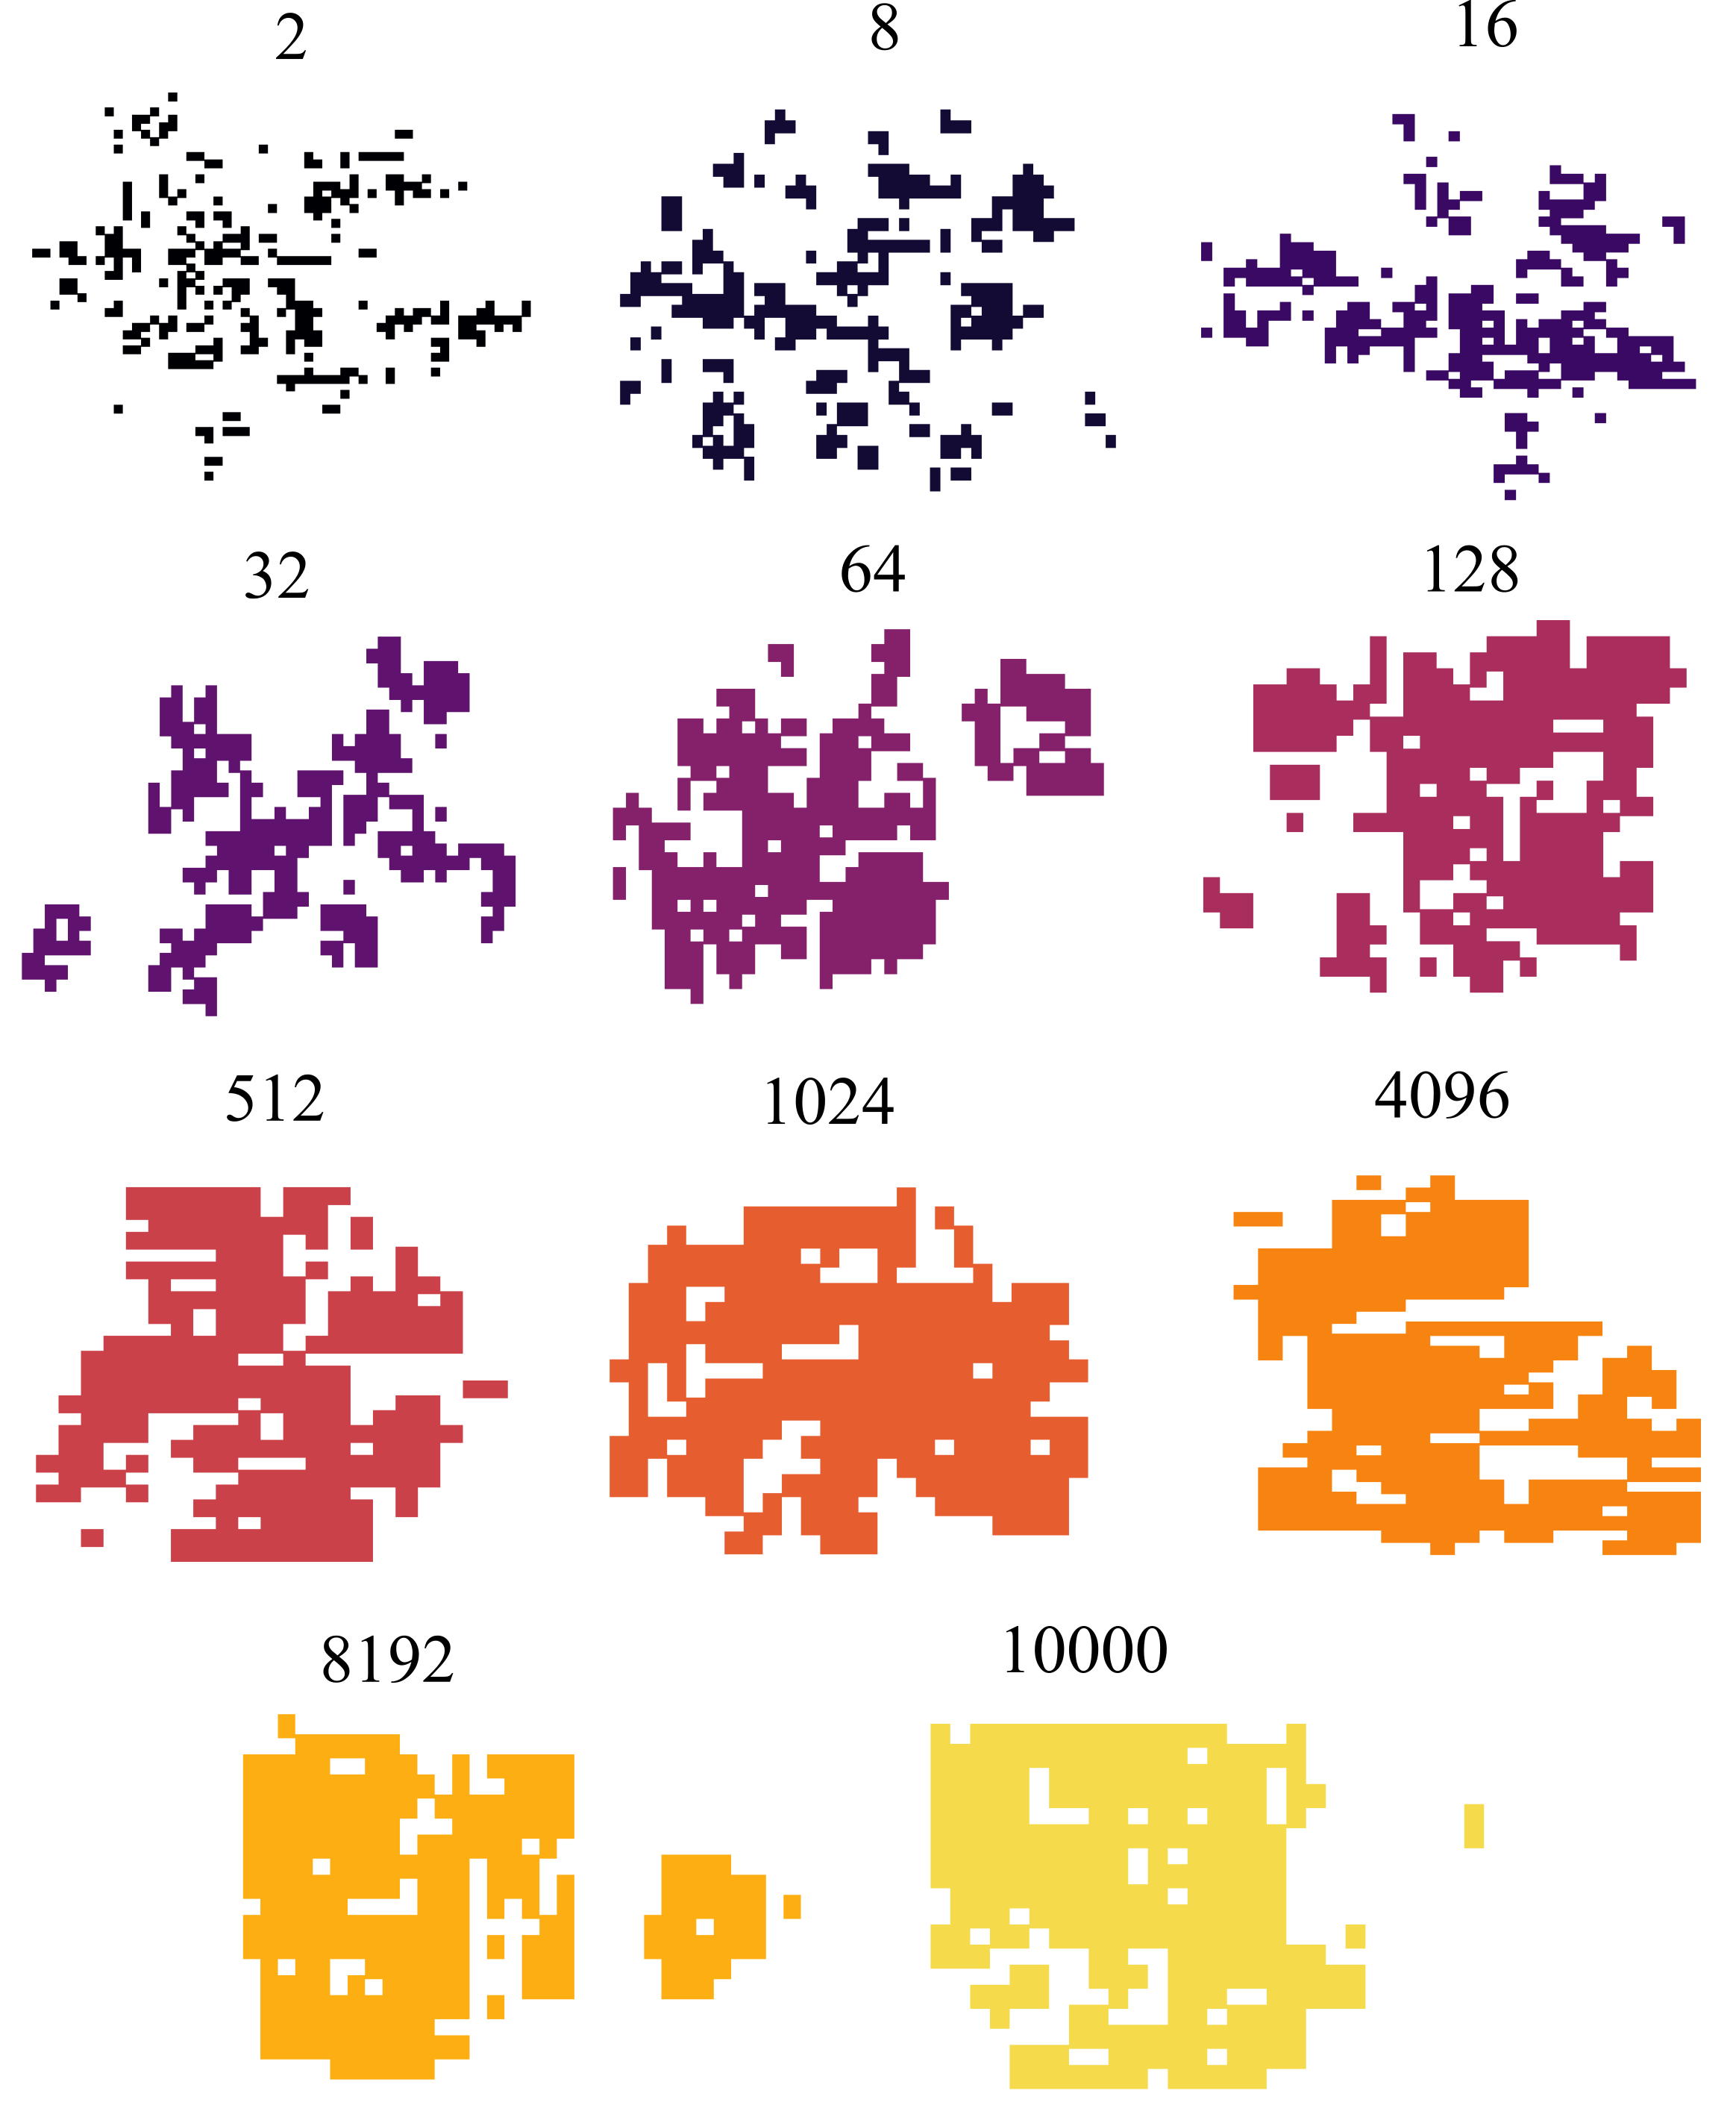
\includegraphics[width=\textwidth]{figures/cs_all.png}
    \caption{Variação da forma da seção transversal das fibrilas para diferentes valores de $T_{s}$.} 
    \label{R3}
\end{figure}

\begin{figure}[H]
    \centering
    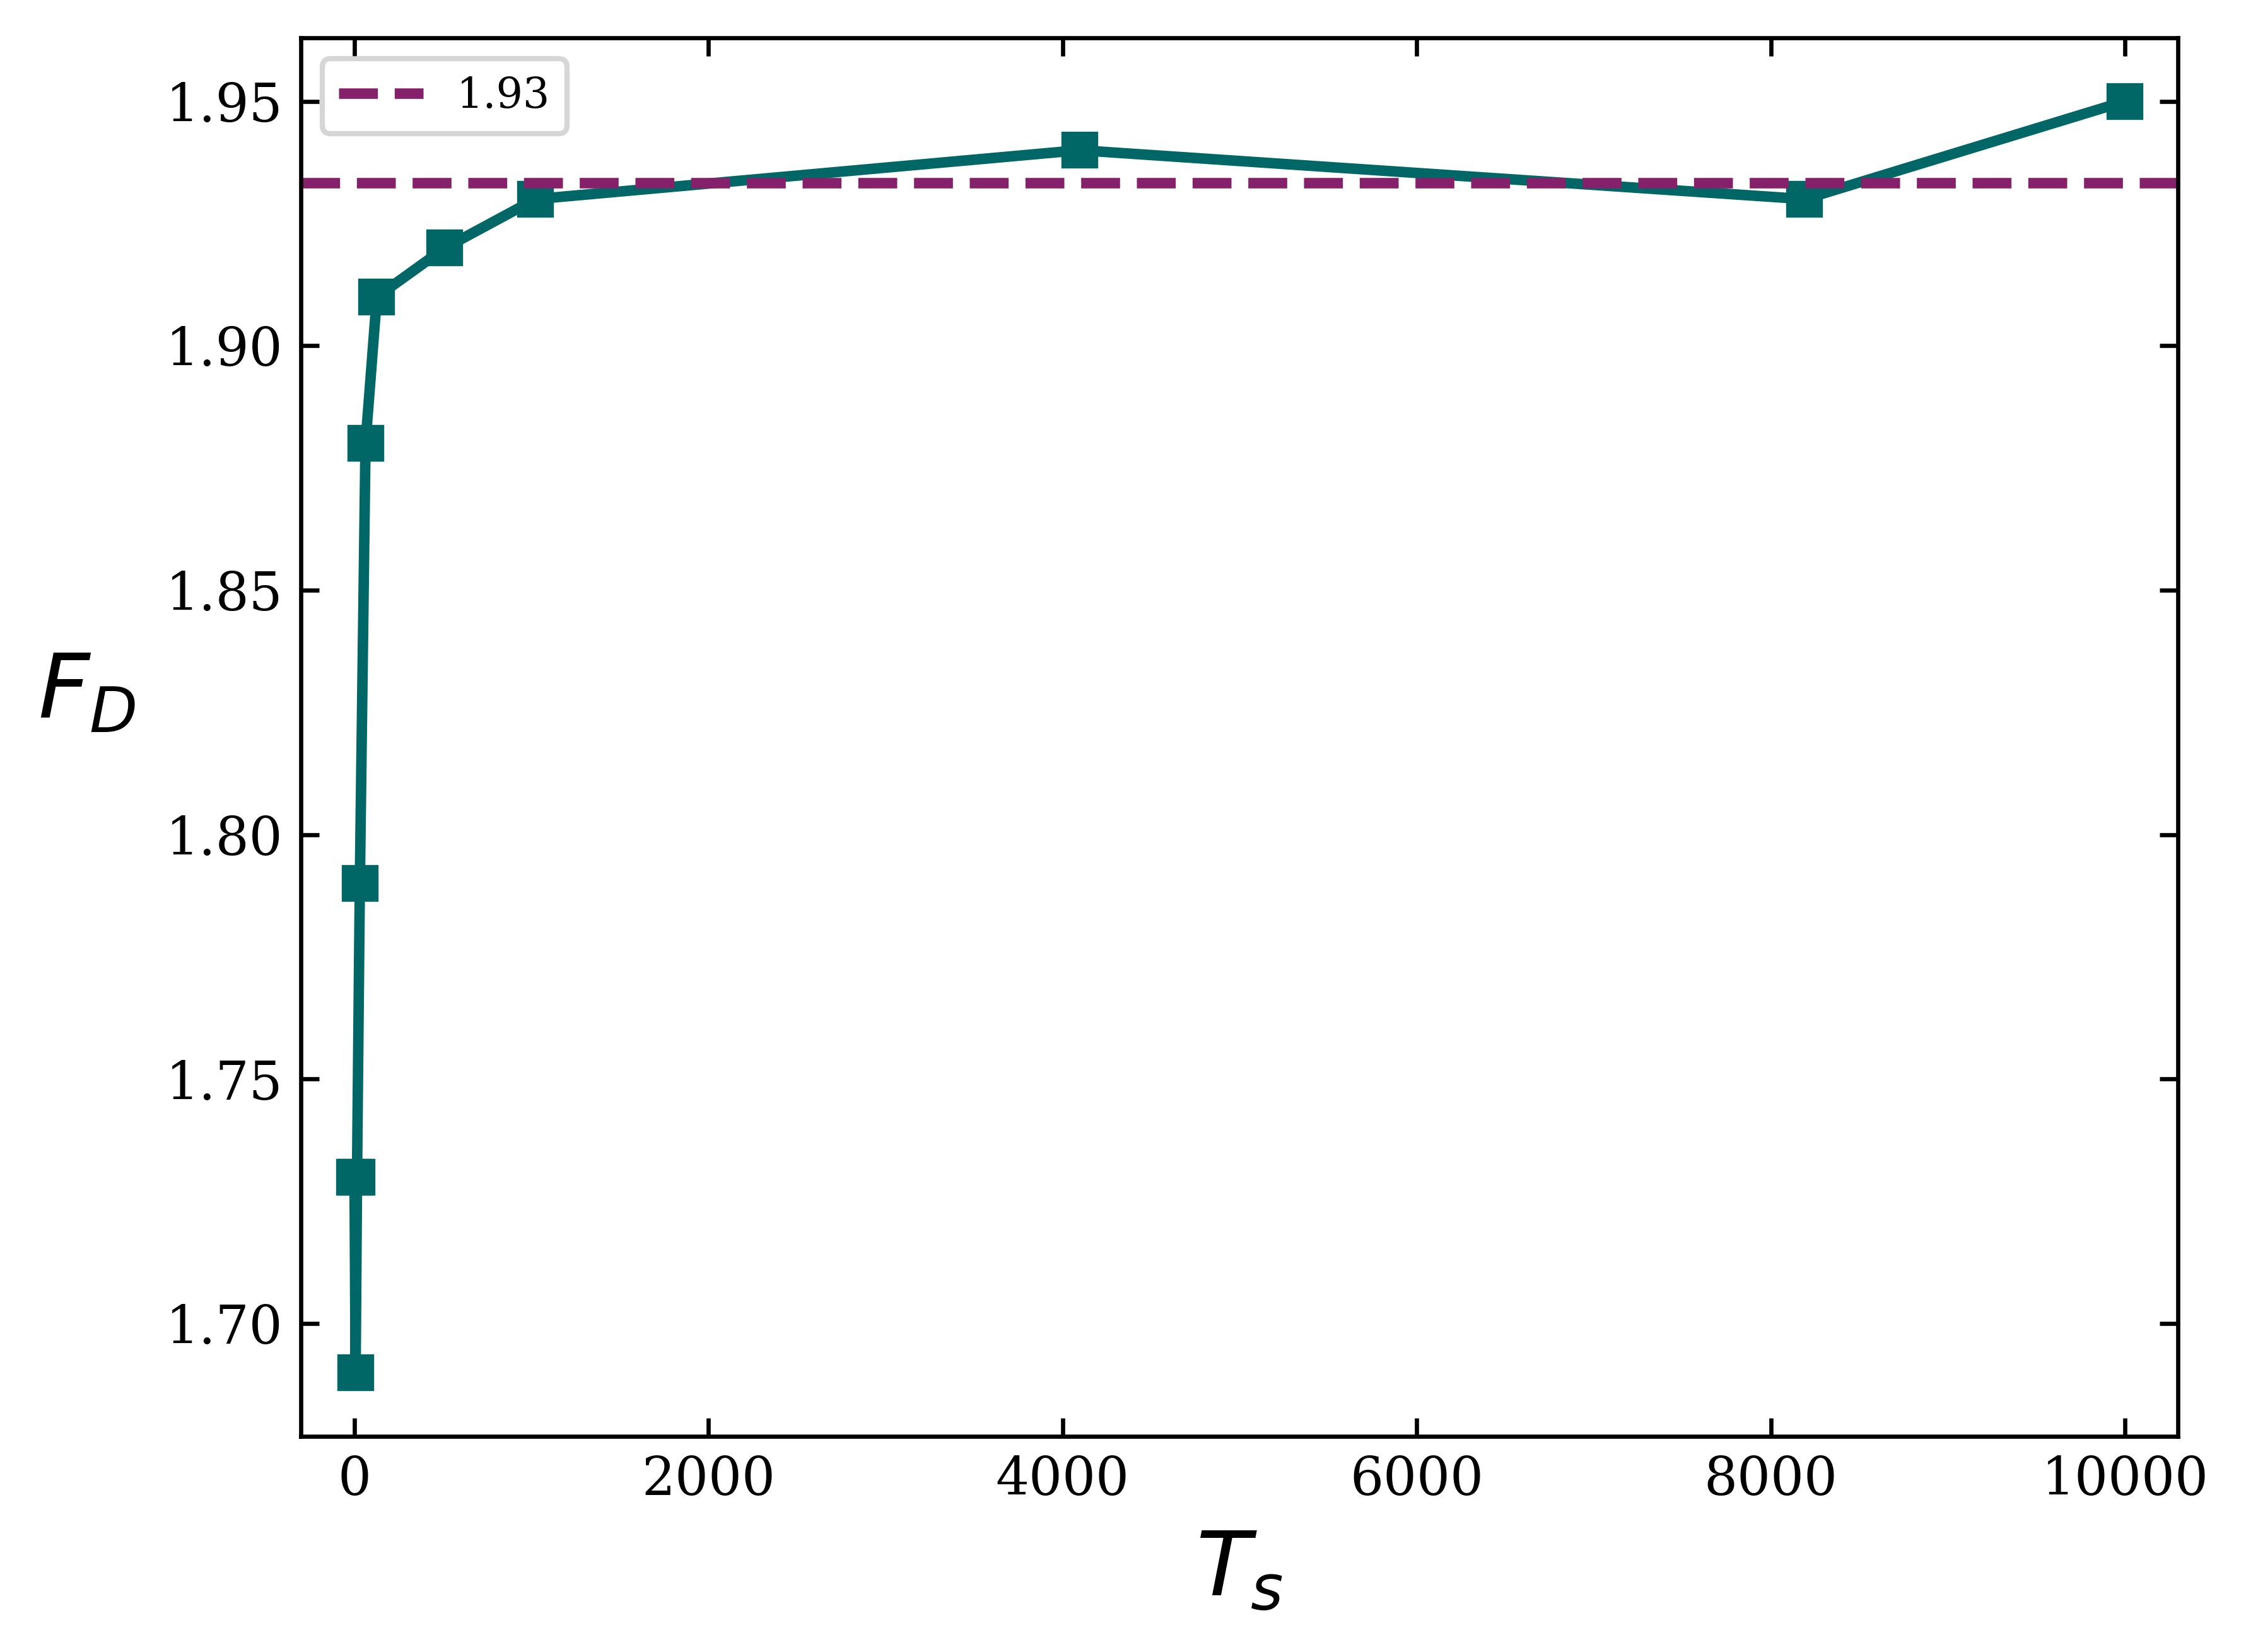
\includegraphics[width=\textwidth]{figures/fd_ts.png}

    \caption{ } 

    \label{R4}
\end{figure}


\subsection{Propriedades mecânicas}

Para entendermos como nosso agregado se comporta mediante a aplicação de uma forca axial, nos avaliamos como o numero de moléculas no agregado varia com a força. Na Figura \ref{R5} temos a curva de stress-strain para fibrilas geradas para diferentes parâmetros $T_{s}$. Nos observamos que, o aumento desse parâmetro influencia no aumento da tensão máxima de ruptura. Contudo, a partir de $T_{s} = $ 512, esse valores se tornam bastante próximos e as curvas se sobrepõem. Normalmente, é esperado que essas curvas cresçam até o valor máximo de uma forma mais abrupta, o que não observamos aqui, mas, esse comportamento suave até o valor limite é consequência do módulo de weibus que utilizamos no modelo, visto que, para valores baixos, a curva resultante é não determinística \cite{Parkinson1997}. 
A tensão máxima suportada que encontramos foi de 45,6 $MPa$. Esse valor é muito próximo ao encontrado nos trabalhos de Yang et al. \cite{YANG2012148} ao analizar fibrilas reconstituídas do tendão de aquiles bovino purificado. No trabalho de Yamamoto \cite{Noritaka}, ele utilizou fibrilas isoladas do fascículo dos tendões da cauda de ratos, obtendo um valor de 100$\pm$ 32 $MPa$. Essa diferença com relação ao nosso valor pode estar relacionada com a dimensão das fibrilas que ele utilizou, visto que elas apresentam um diâmetro muito maior do que as modeladas nesse trabalho.

\begin{figure}[H]
    \centering
    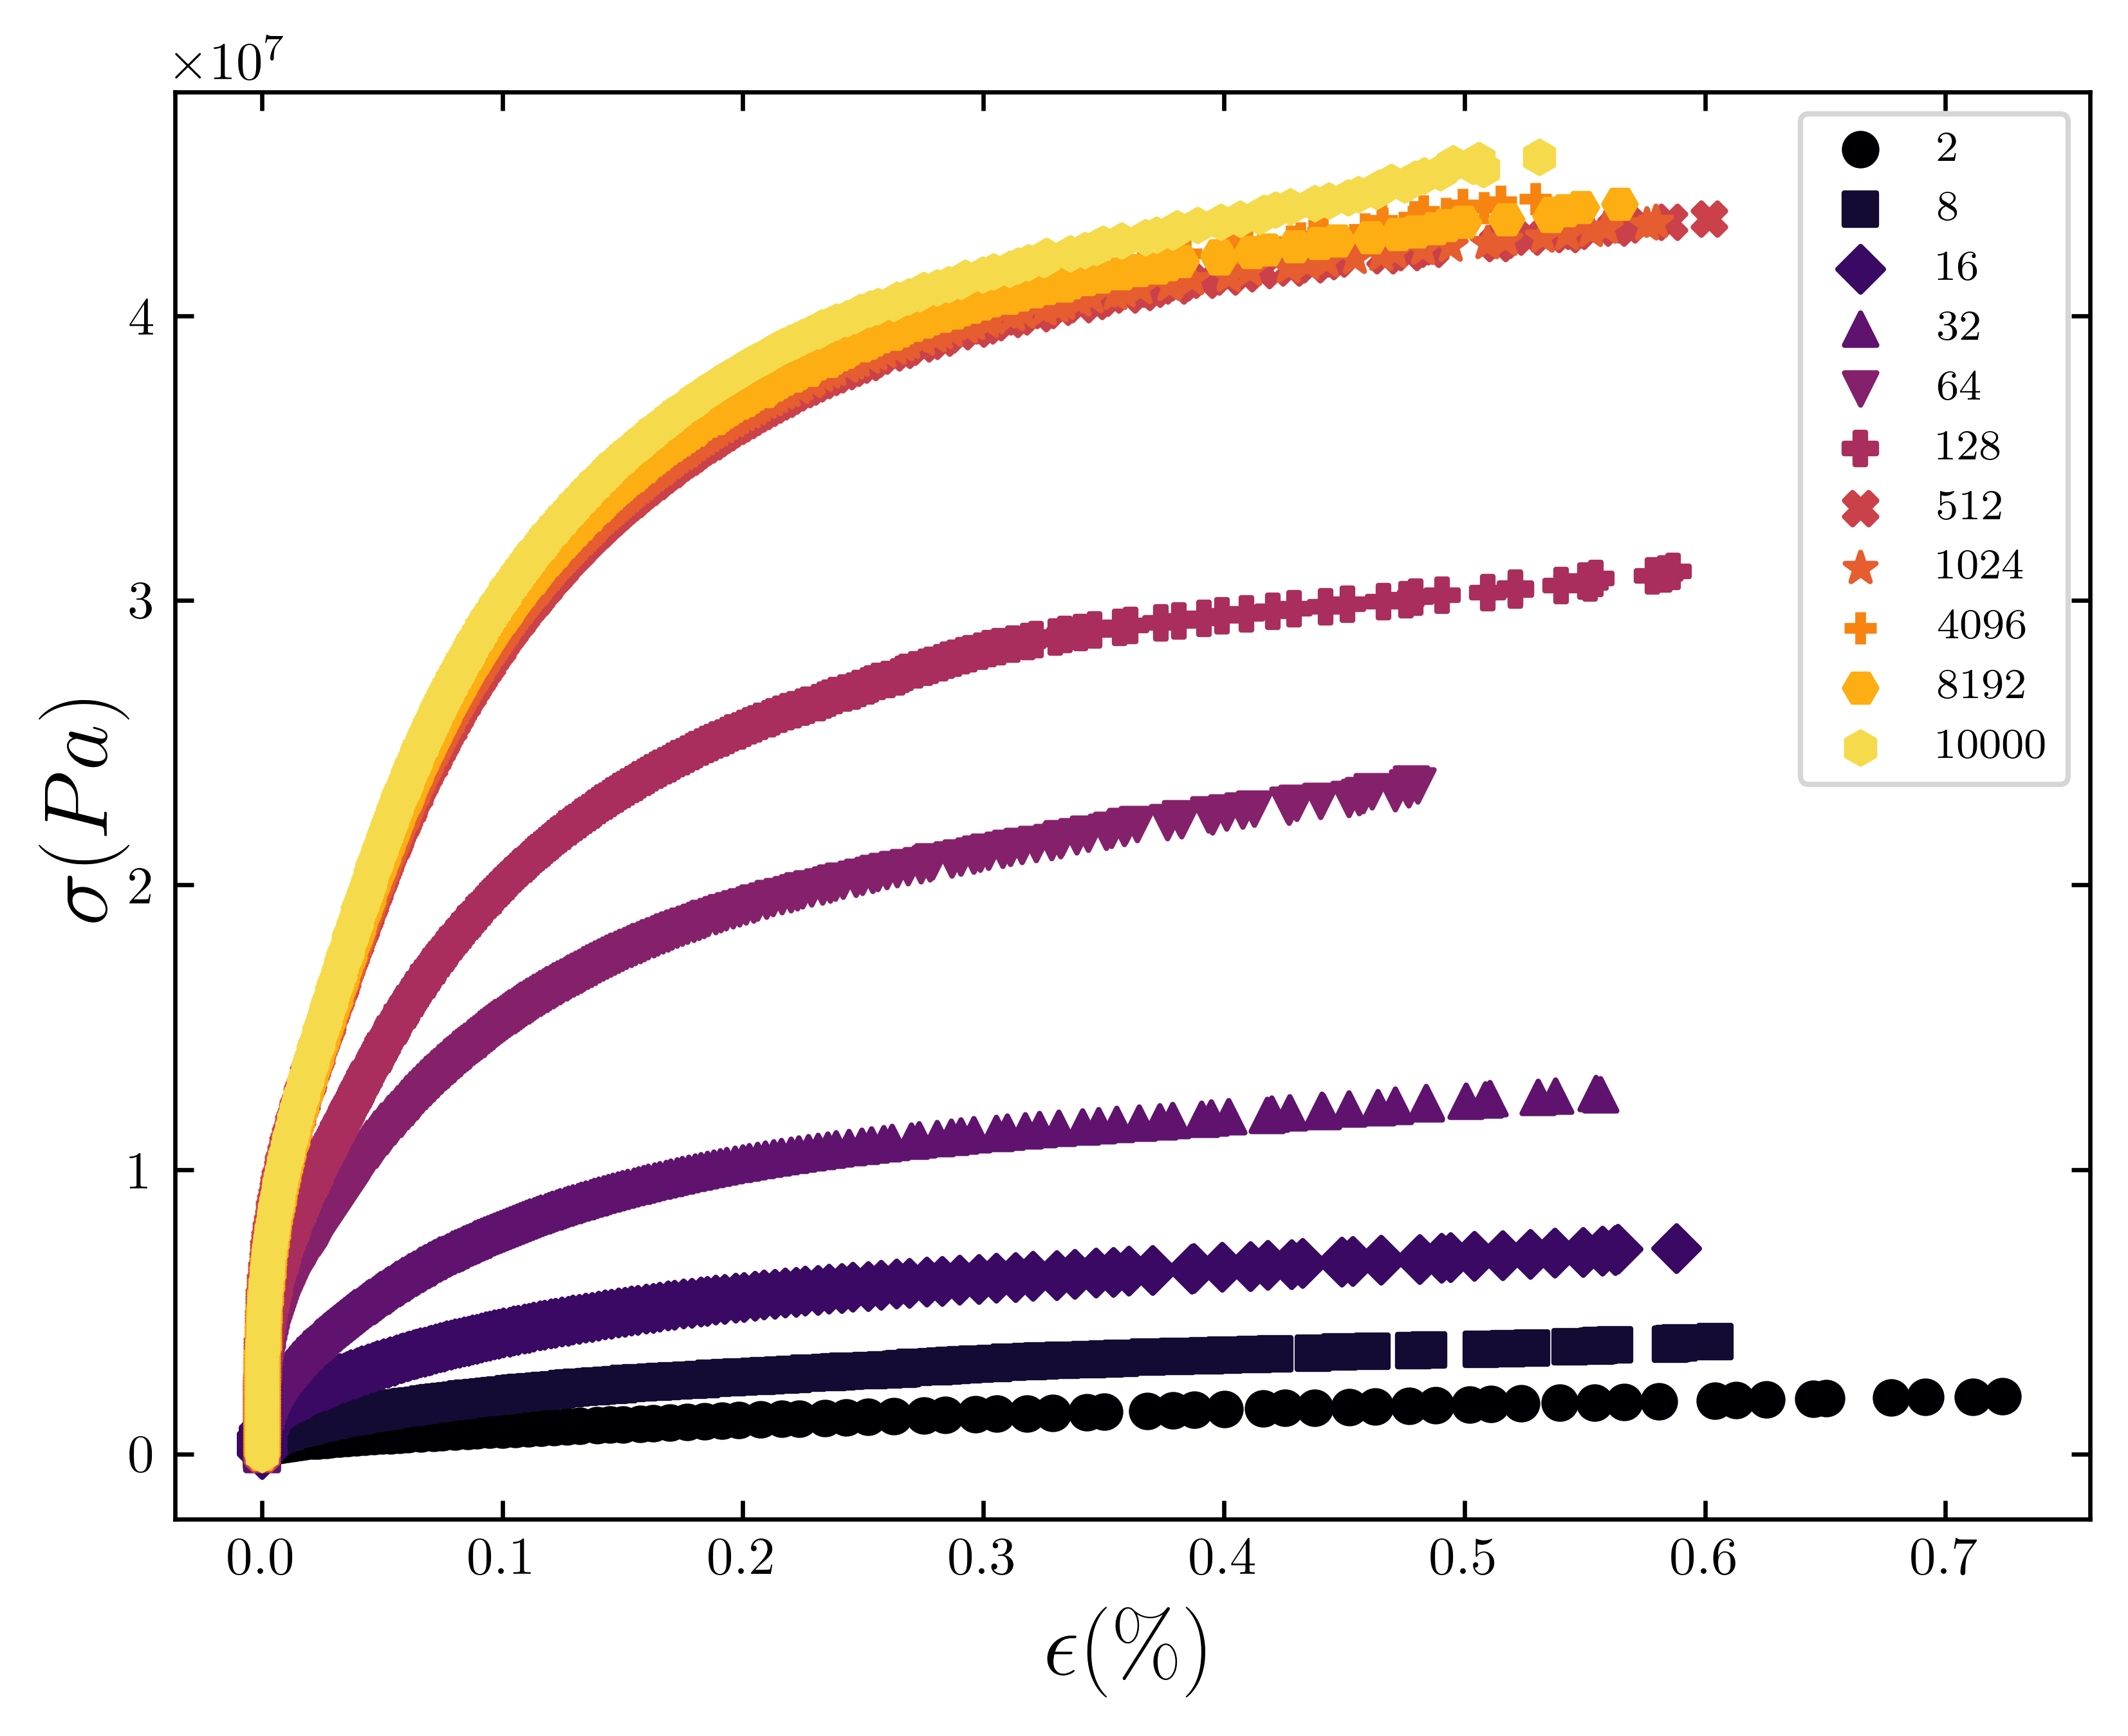
\includegraphics[width=\textwidth]{figures/stress_strain.png}

    \caption{Tensão em função da deformação da fibrila para diferentes valores de $T_{s}$.} 

    \label{R5}
\end{figure}

Na Figura \ref{R6}, podemos observar como os valores de tensão máxima suportada variam com um importante parâmetro das fibrilas, a densidade. 
Nos escolhemos essa analise visto que o comportamento de $\sigma$ e da densidade, $\rho$, possuem a mesma forma quando em função do $T_{s}$. Nos identificamos um comportamento exponencial para o aumento da tensão máxima até um limite superior de 44,1 $MPa$. 
A saturação da densidade ocorre para 66$\%$, bem próximo ao encontrado nos trabalho de Parkinson et al\cite{Parkinson1995} com esse modelo, mas um tanto abaixo do valor determinados por Katz et al\cite{KATZ1973351}, que calculou experimentalmente como 80$\%$ de espaço disponível ocupado para as fibrilas de colágeno. A partir dessa característica, se mostra uma opção, visto que o tempo computacional é um recurso caro, que esse modelo pode ser rodado, para os parâmetros que usamos inicialmente, com $T_{s}=$ 512, uma vez que é onde já obtemos fibrilas com os valores de interesse, em média, iguais para valores superiores desse parâmetro.



\begin{figure}[H]
    \centering
    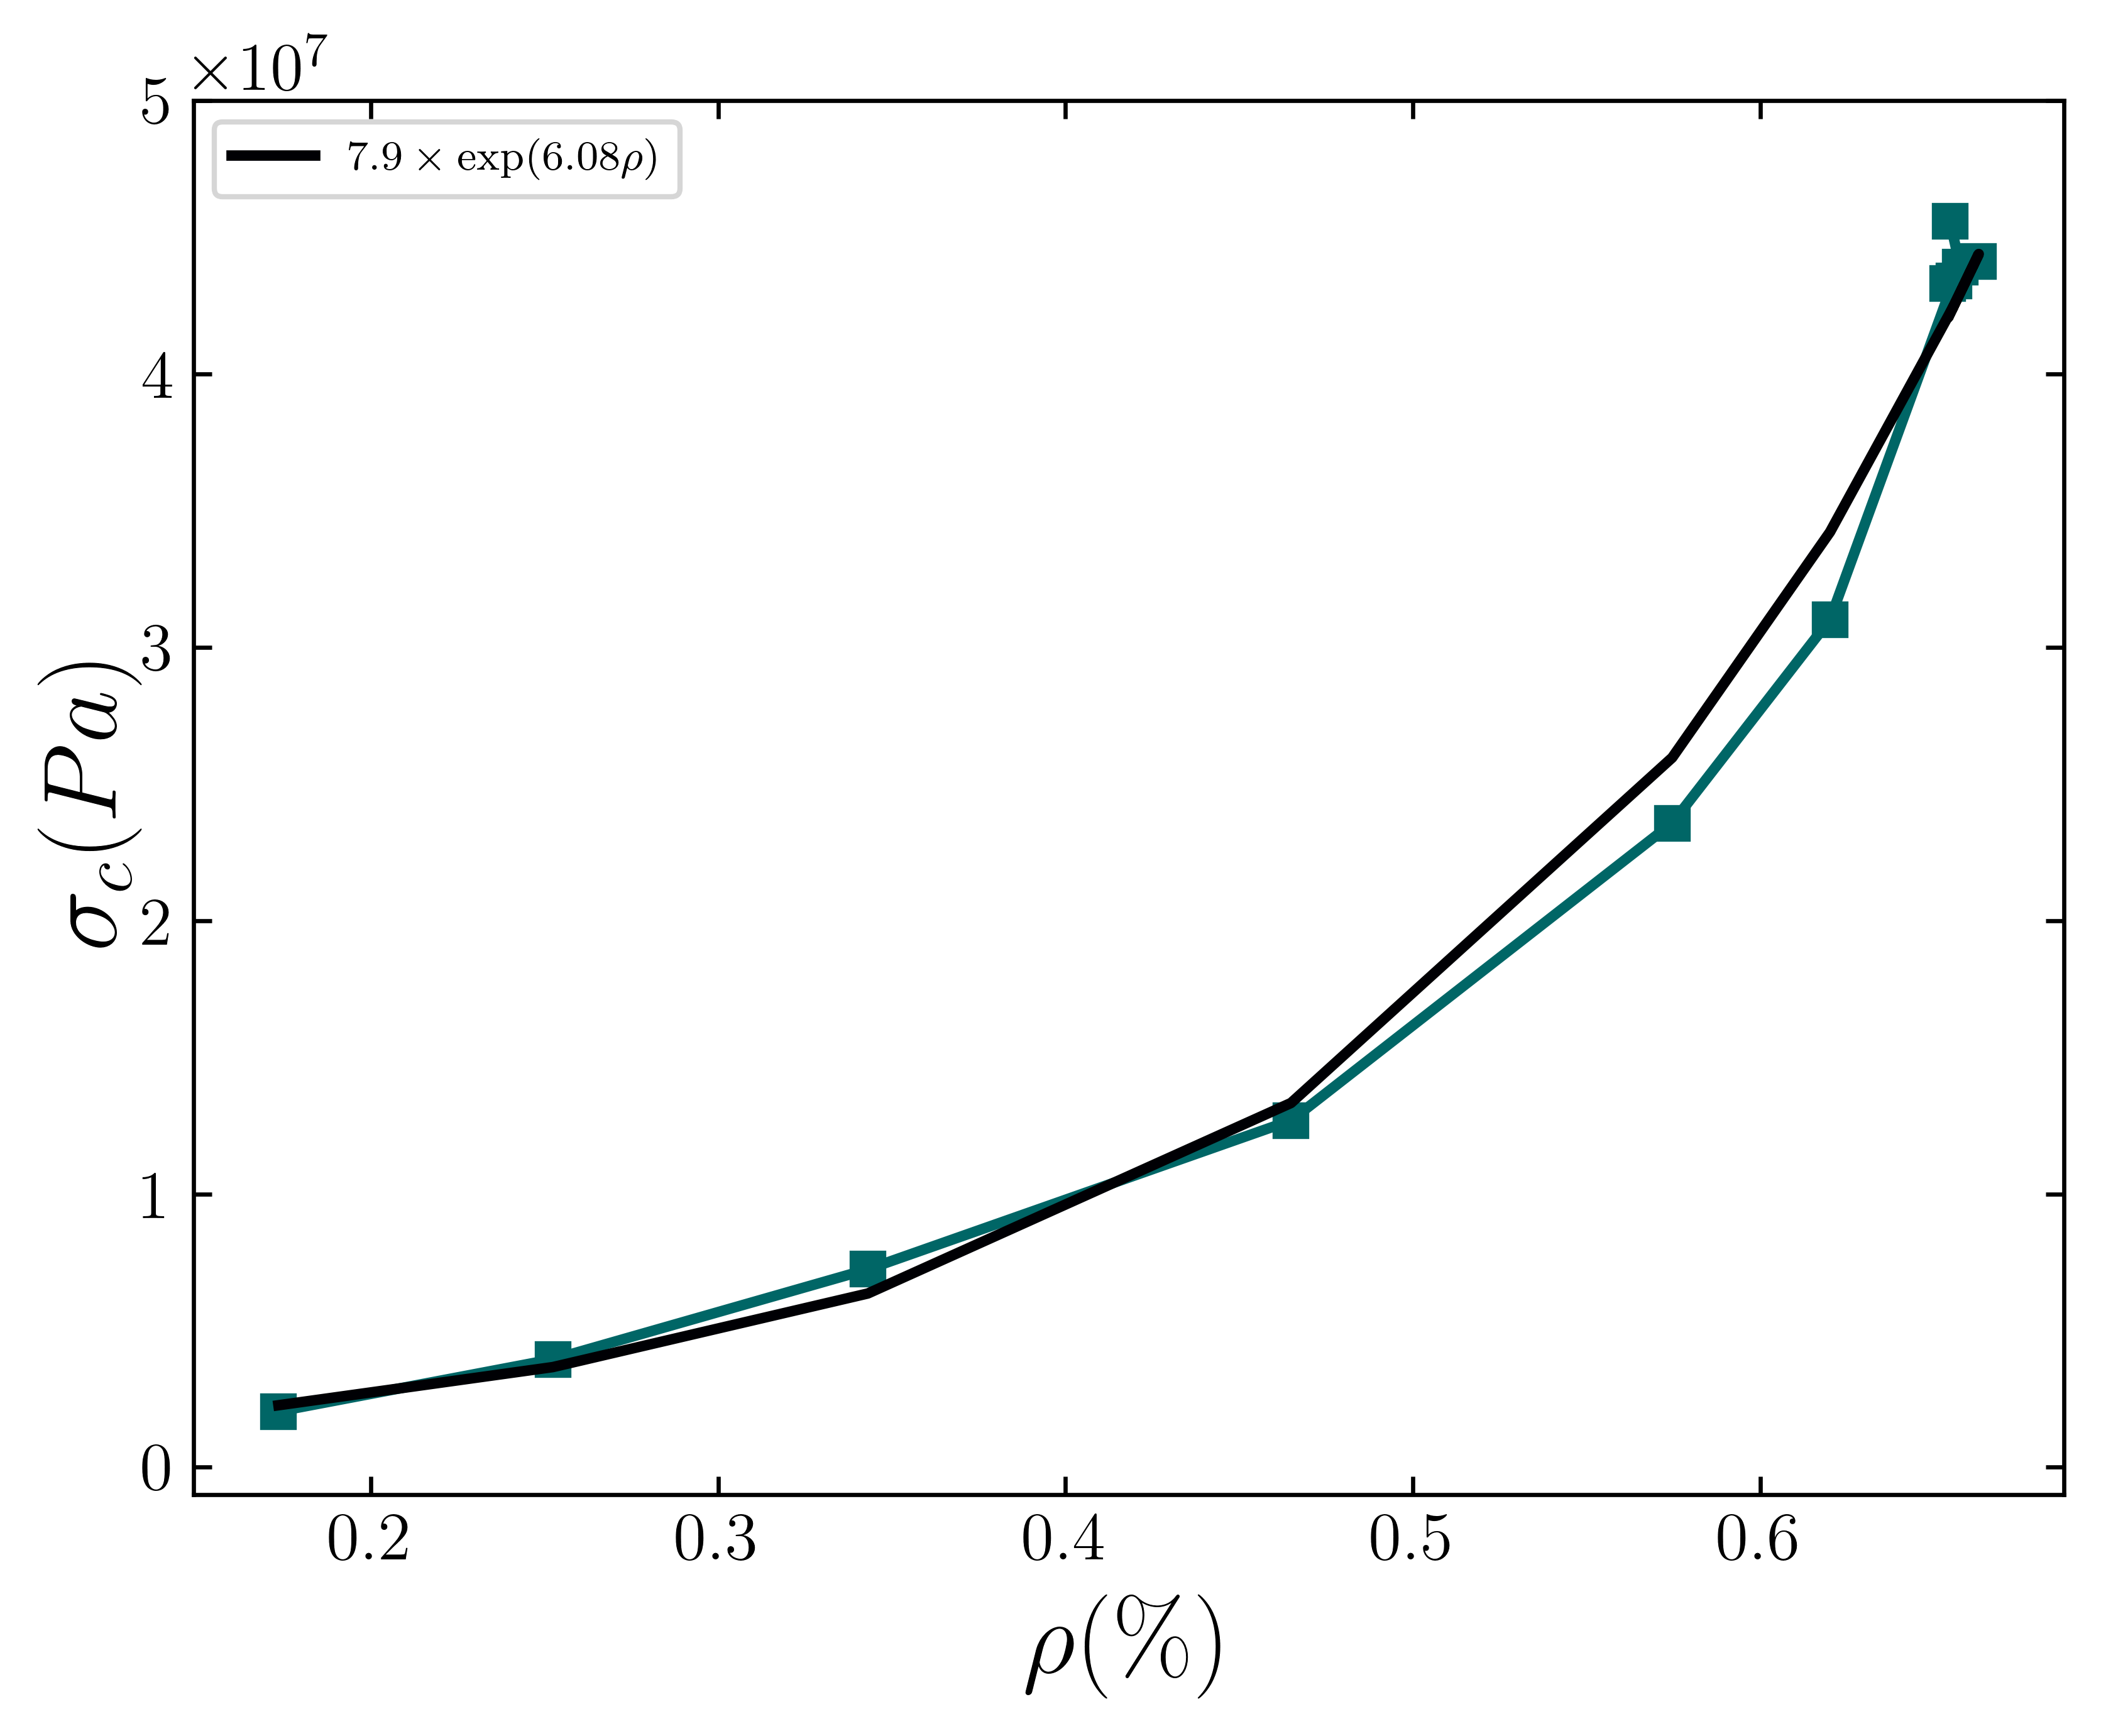
\includegraphics[width=\textwidth]{figures/sigma_rho.png}

    \caption{Tensão crítica em função da densidade. Observamos que esse valor cresce exponencialmente com a densidade até ambos os parâmetros atingirem um limite superior.} 


    \label{R6}
\end{figure}

Ao analisar como o processo de ruptura ocorria no nosso modelo, bem como em outros, vimos que a redistribuição de tensão, para uma mesma força
poderia levar a ocorrencia de ruptura em cascata. Na Figura \ref*{R7}, temos a distribuição das avalanches de ruptura em função do seu tamanho.
Podemos observar a existeencia de duas ordens de grandeza bem definidas, após isso, os dados sofrem com efeito de tamanho.
Analizando a região de interesse, conseguimos determinar o expoente das leis de escala de modo que,
eles crescem com o aumento do parâmetro $T_{s}$, contudo, podemos notar que rapidamente as curvas de
avalanche se superpoem muito rapidamente, indicando que o processo de ruptura é praticamente o mesmo
para diferentes valores do parâmetro. 




\begin{figure}[H]
    \centering
    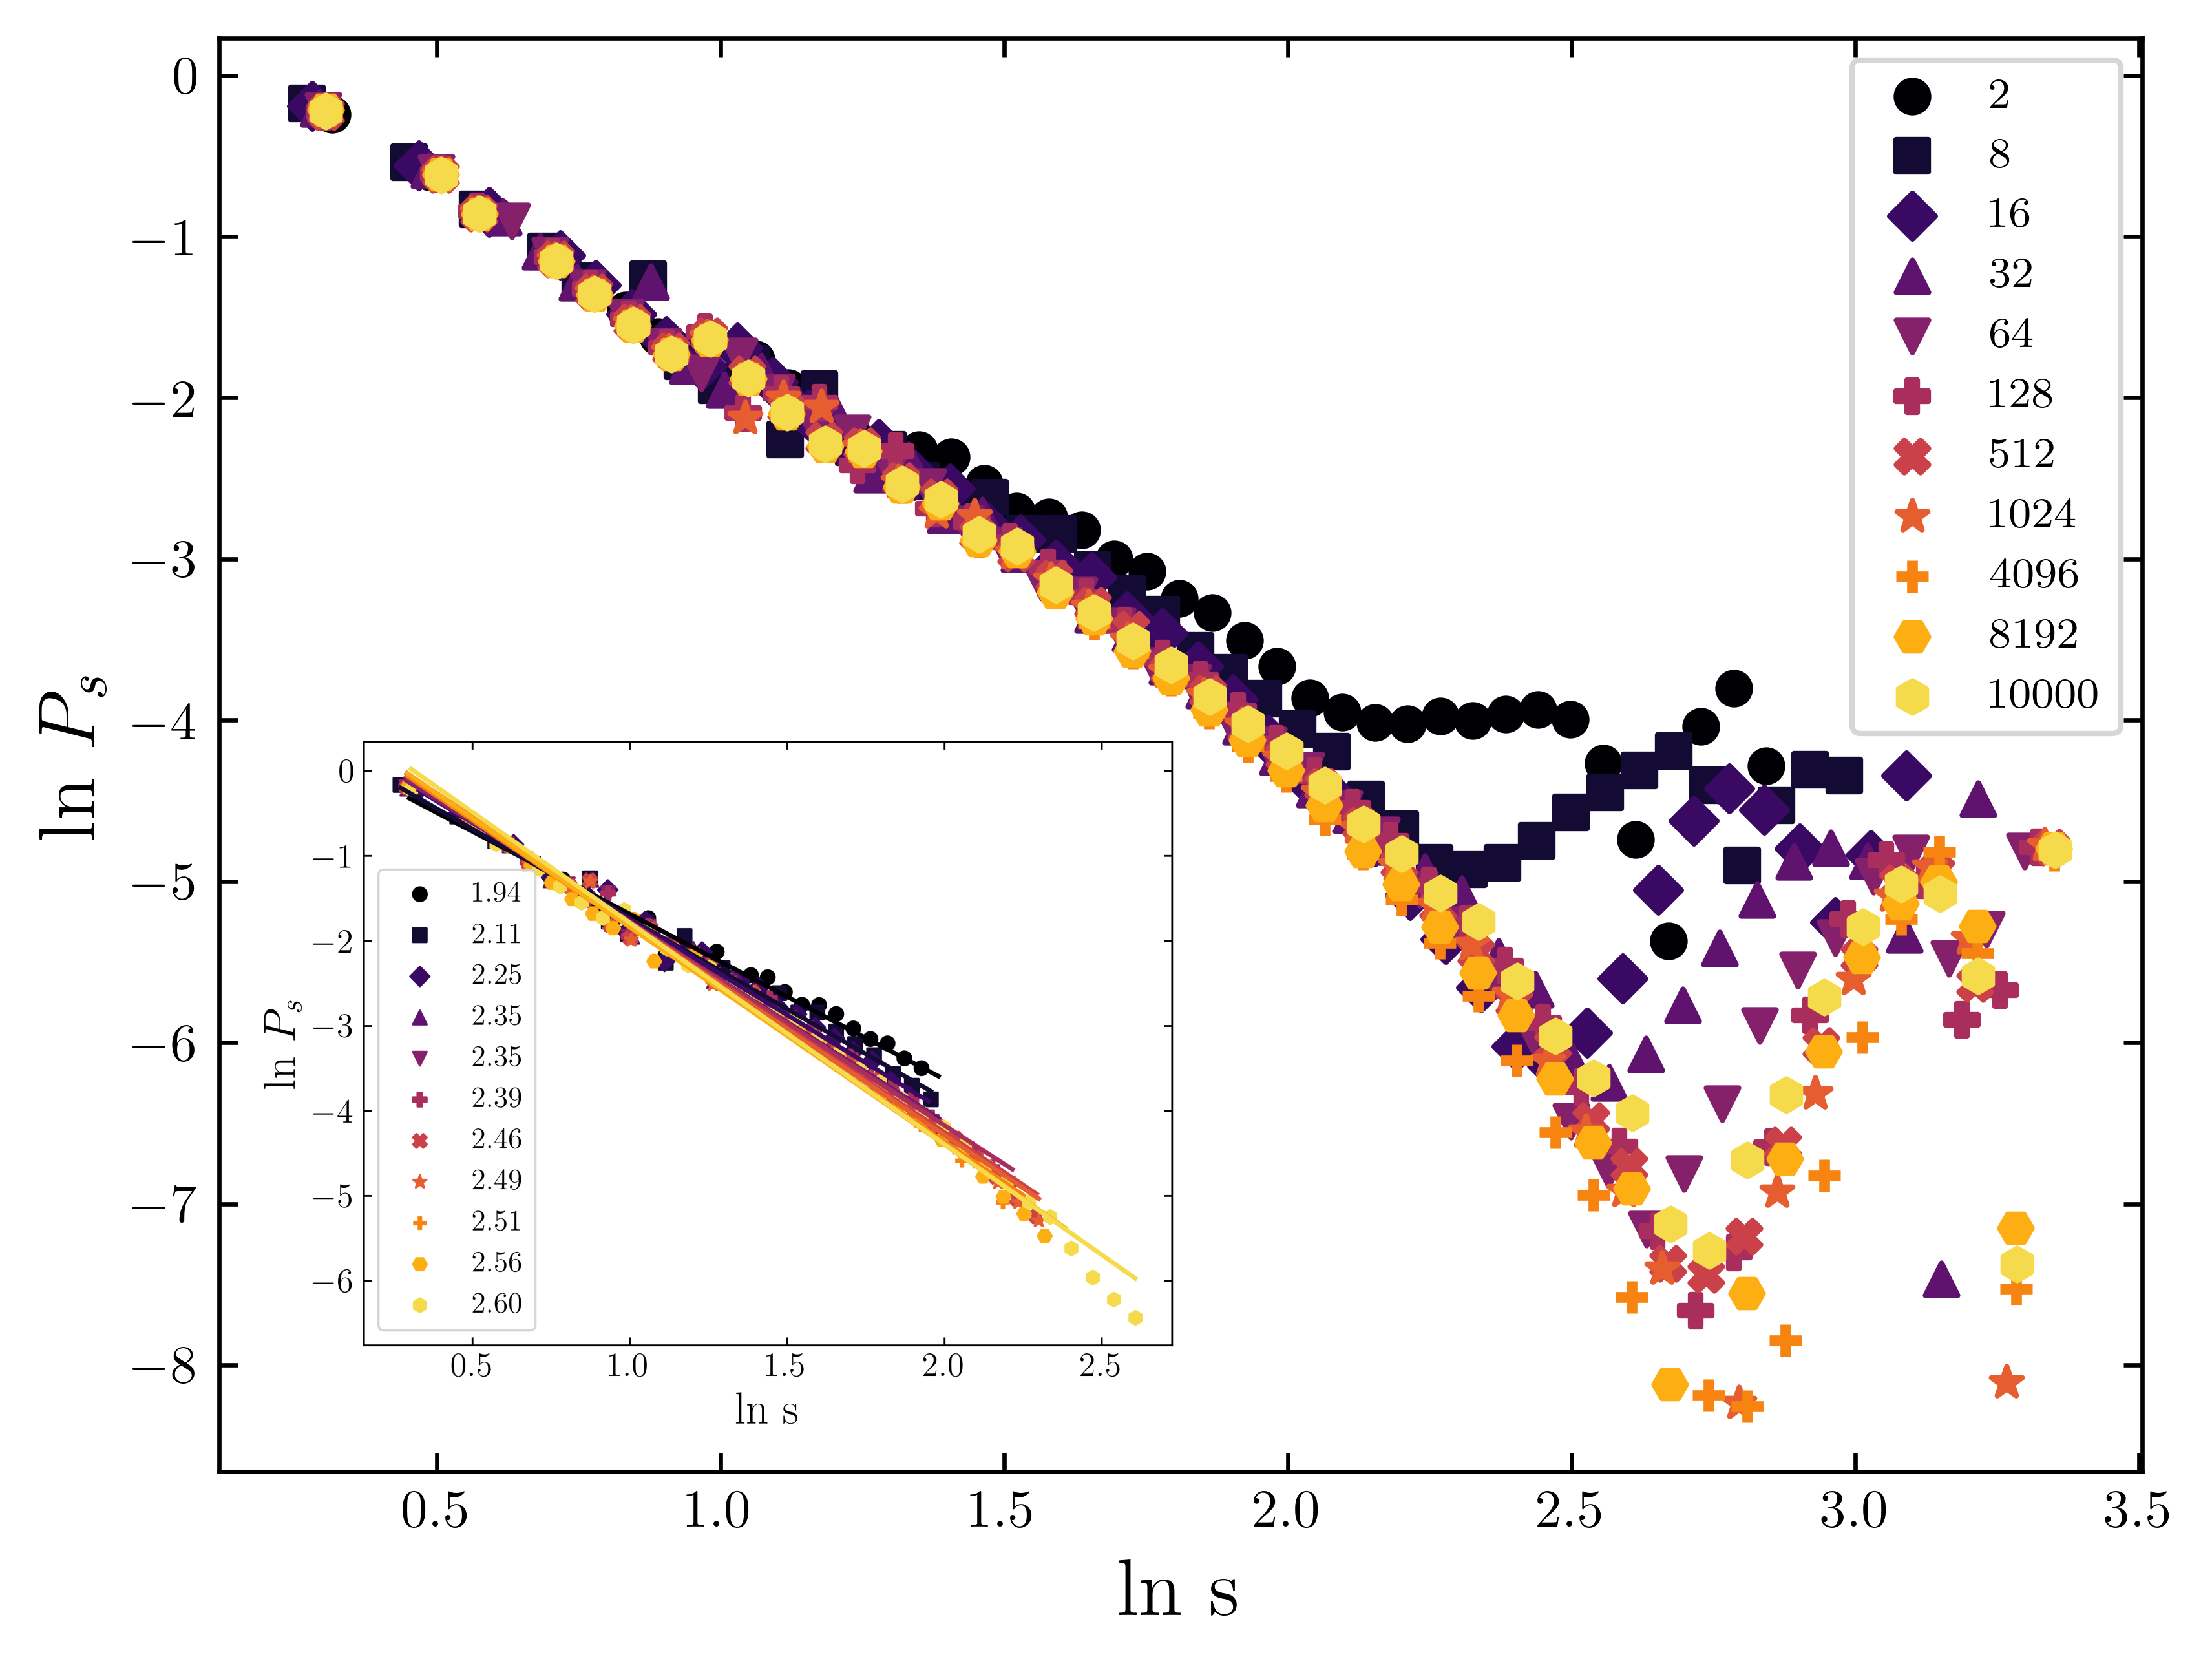
\includegraphics[width=\textwidth]{figures/ava.png}

    \caption{} 

    \label{R7}
\end{figure}










\begin{figure}[H]
    \centering
    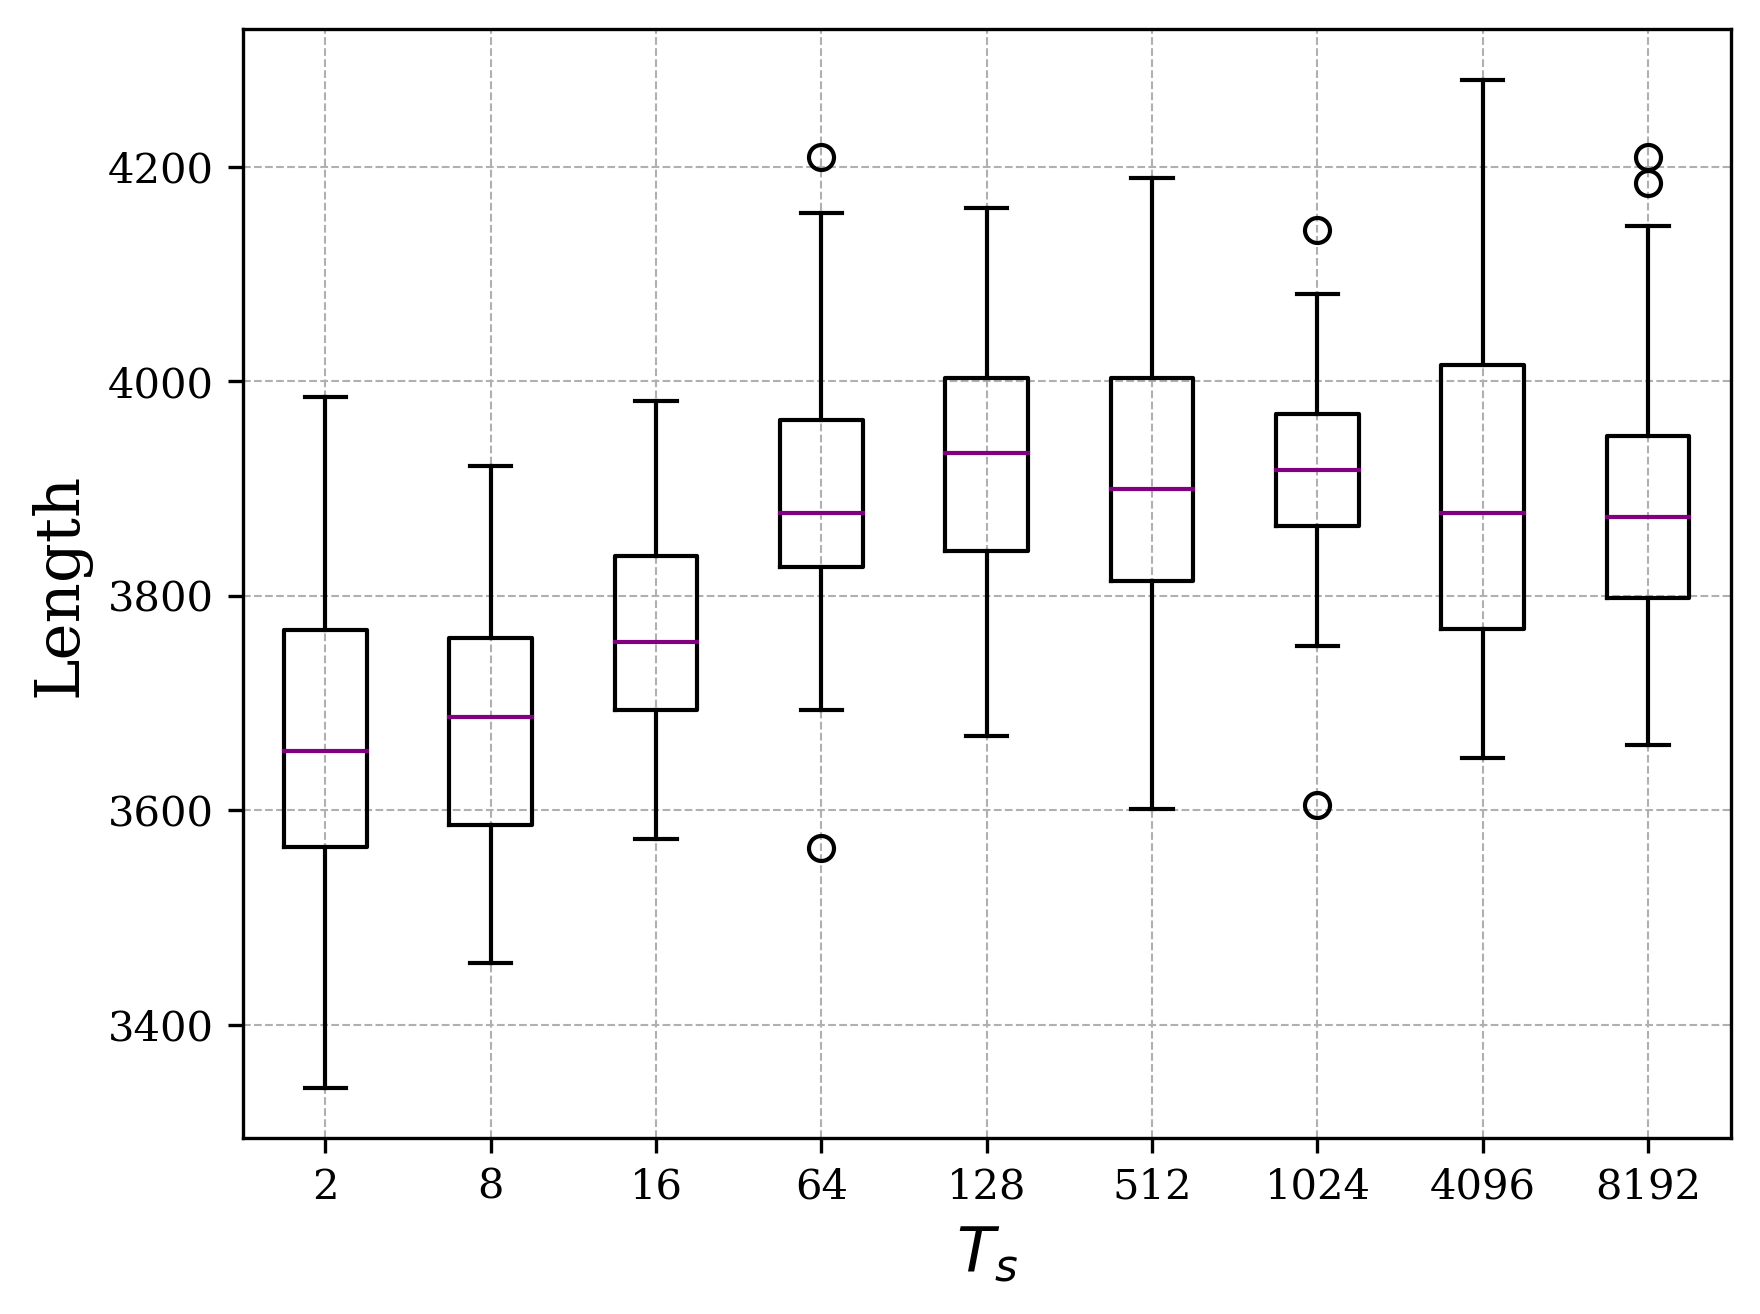
\includegraphics[width=\textwidth]{figures/box_plot_length.png}

    \caption{Por ser um processo estocástico, temos que o comprimento das fibrilas, em função do $T_{s}$, apresenta uma variabilidade com poucos outfits. Tomando o comprimento médio, temos que existe uma tendência de crescimento à medida que o parâmetro $T_{s}$ aumenta; após esse valor, parece haver uma tendência de flutuação desses comprimentos em torno de uma média.} 

    \label{}
\end{figure}

\begin{figure}[h]
    \centering
    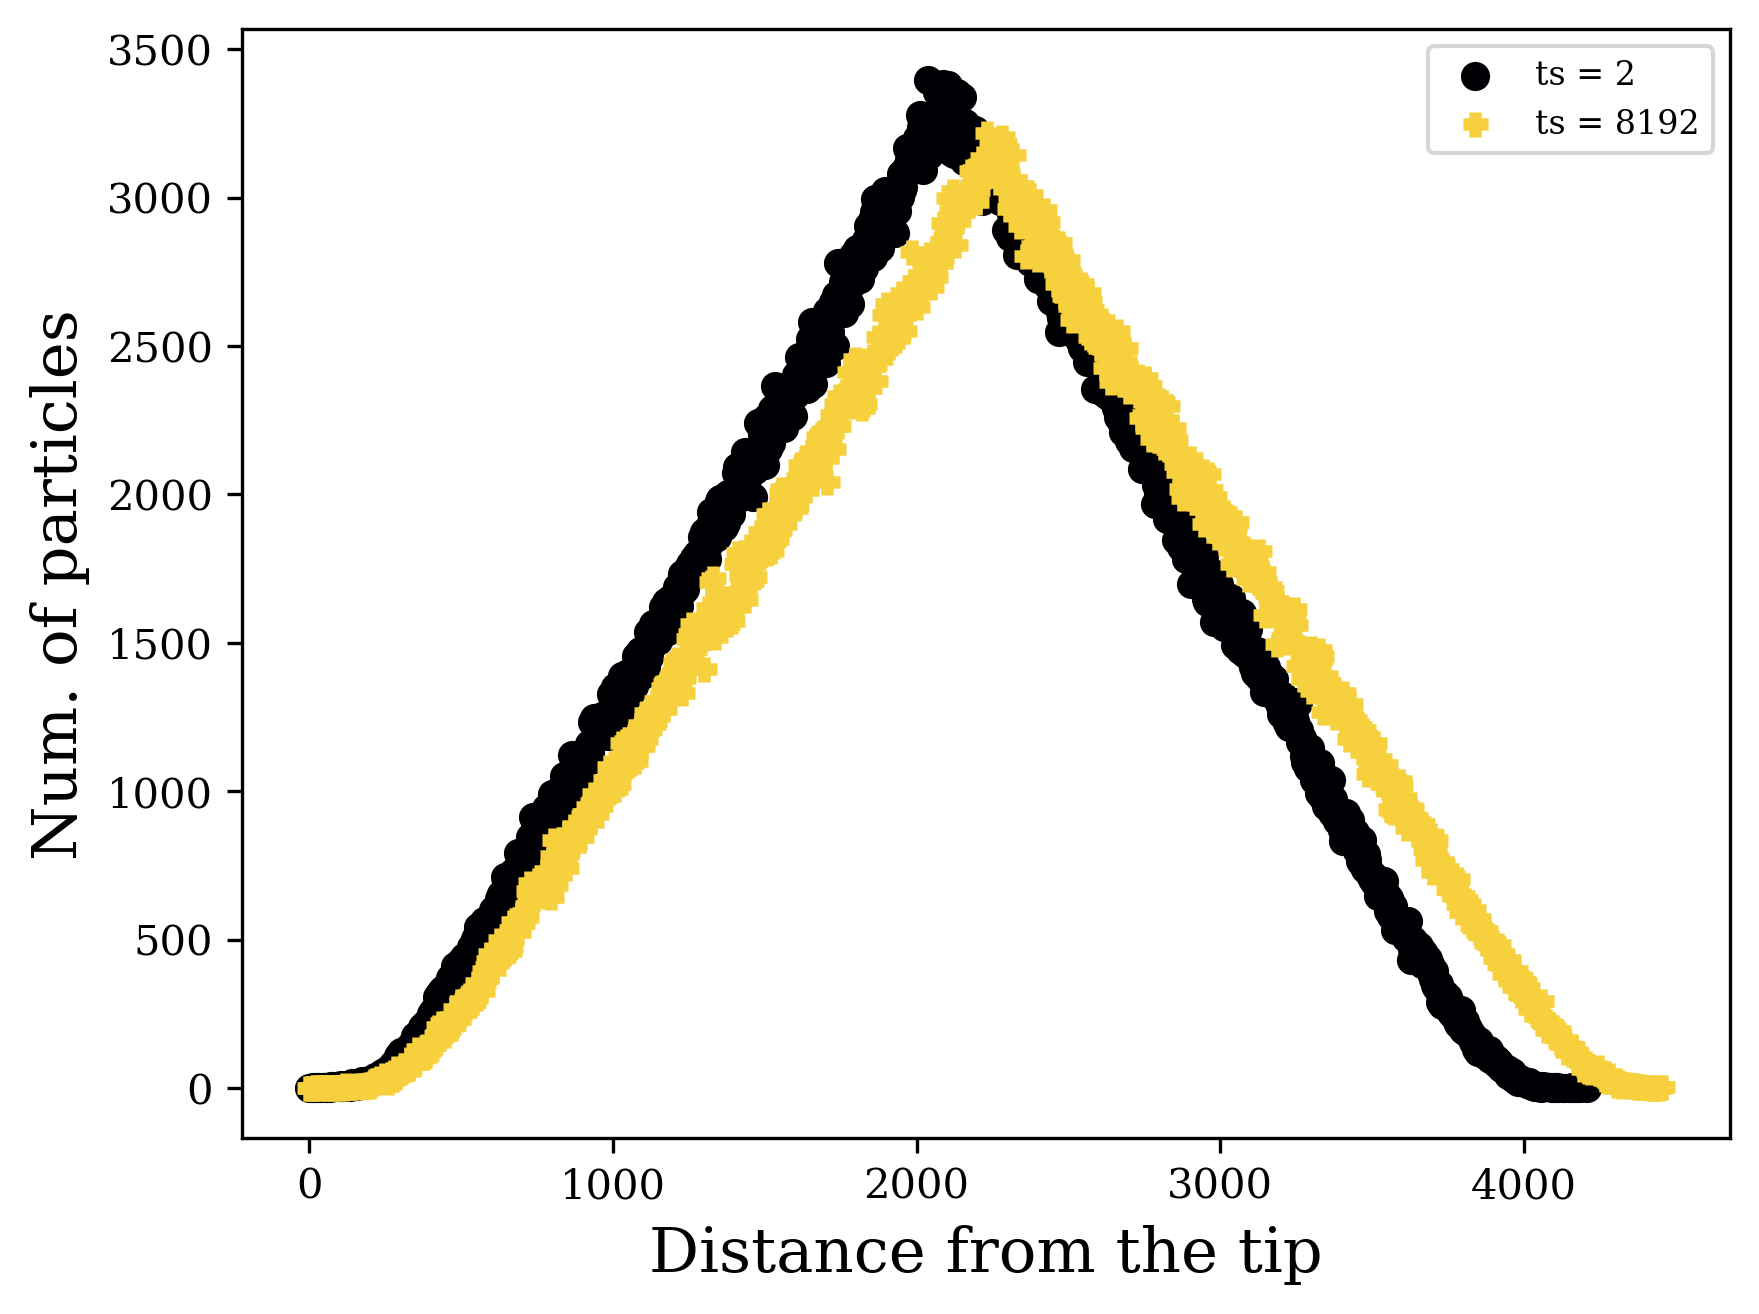
\includegraphics[width=\textwidth]{figures/particles_distance.png}

    \caption{As fibrilas apresentam um comportamento linear na relação massa em função da distância as pontas. À medida que nos afastamos de uma das extremidades, a massa na seção transversal tende a crescer até um pico na região próximo ao centro da fibrila. À medida que nos afastamos, o comportamento inverso acontece. Na figura, temos esse comportamento observado para $T_{s} = 2 $ e $T_{s} =8192$, contudo, esse comportamento se apresenta o mesmo para os outros valores do parâmetro.} 

    \label{}
\end{figure}

\begin{figure}[H]
    \centering
    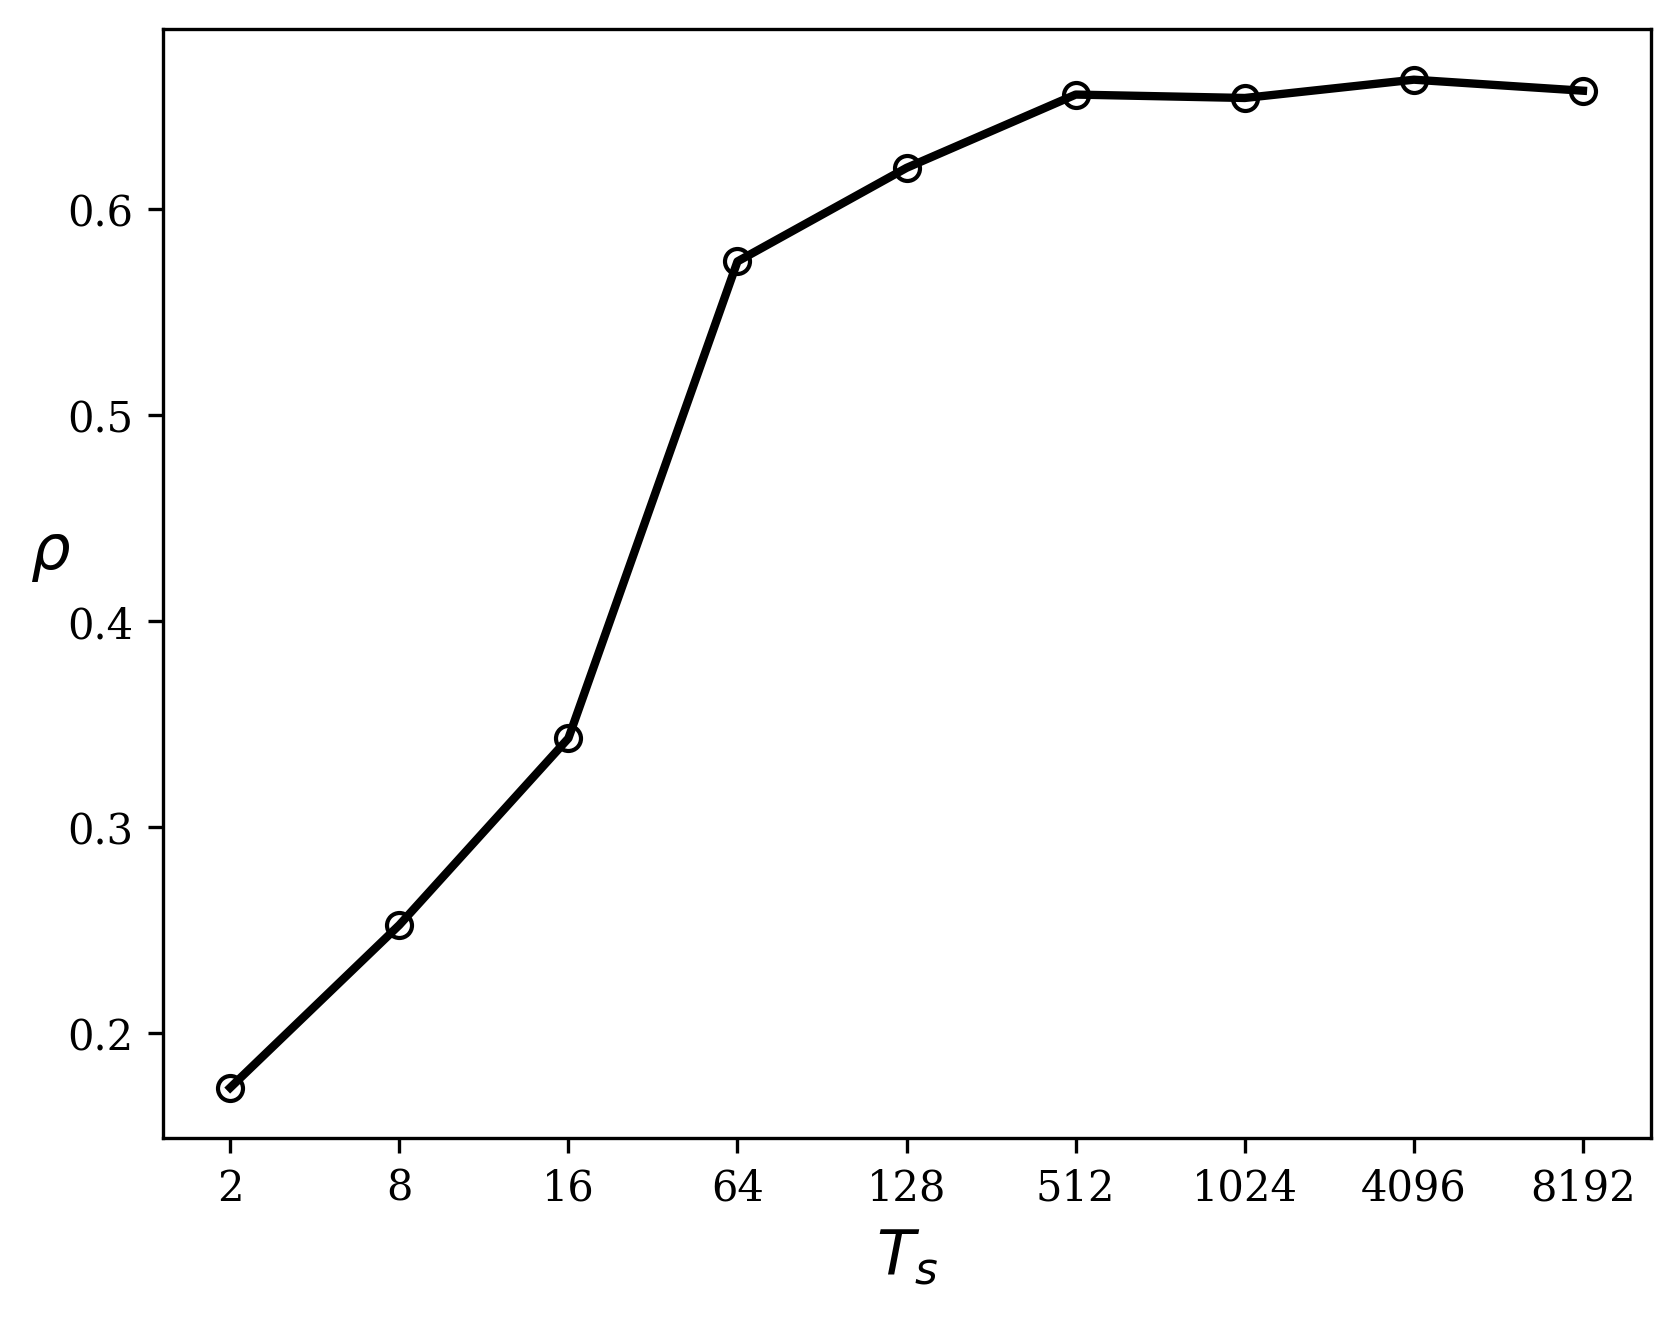
\includegraphics[width=\textwidth]{figures/dens_ts.png}

    \caption{Ao analisarmos a densidade do esqueleto ativo, podemos perceber que ela cresce com o parâmetro $T_{s}$. A curva parece atingir um platô para $T_{s} >= 512$. Nessa região, em média, a densidade do esqueleto é de $65\%$ do volume possível. Esse comportamento mostra que certos valores de $T_{s}$, muito altos, esse parâmetro não exerce mais efeito sobre a densidade.} 

    \label{}
\end{figure}





\begin{figure}[H]
    \centering
    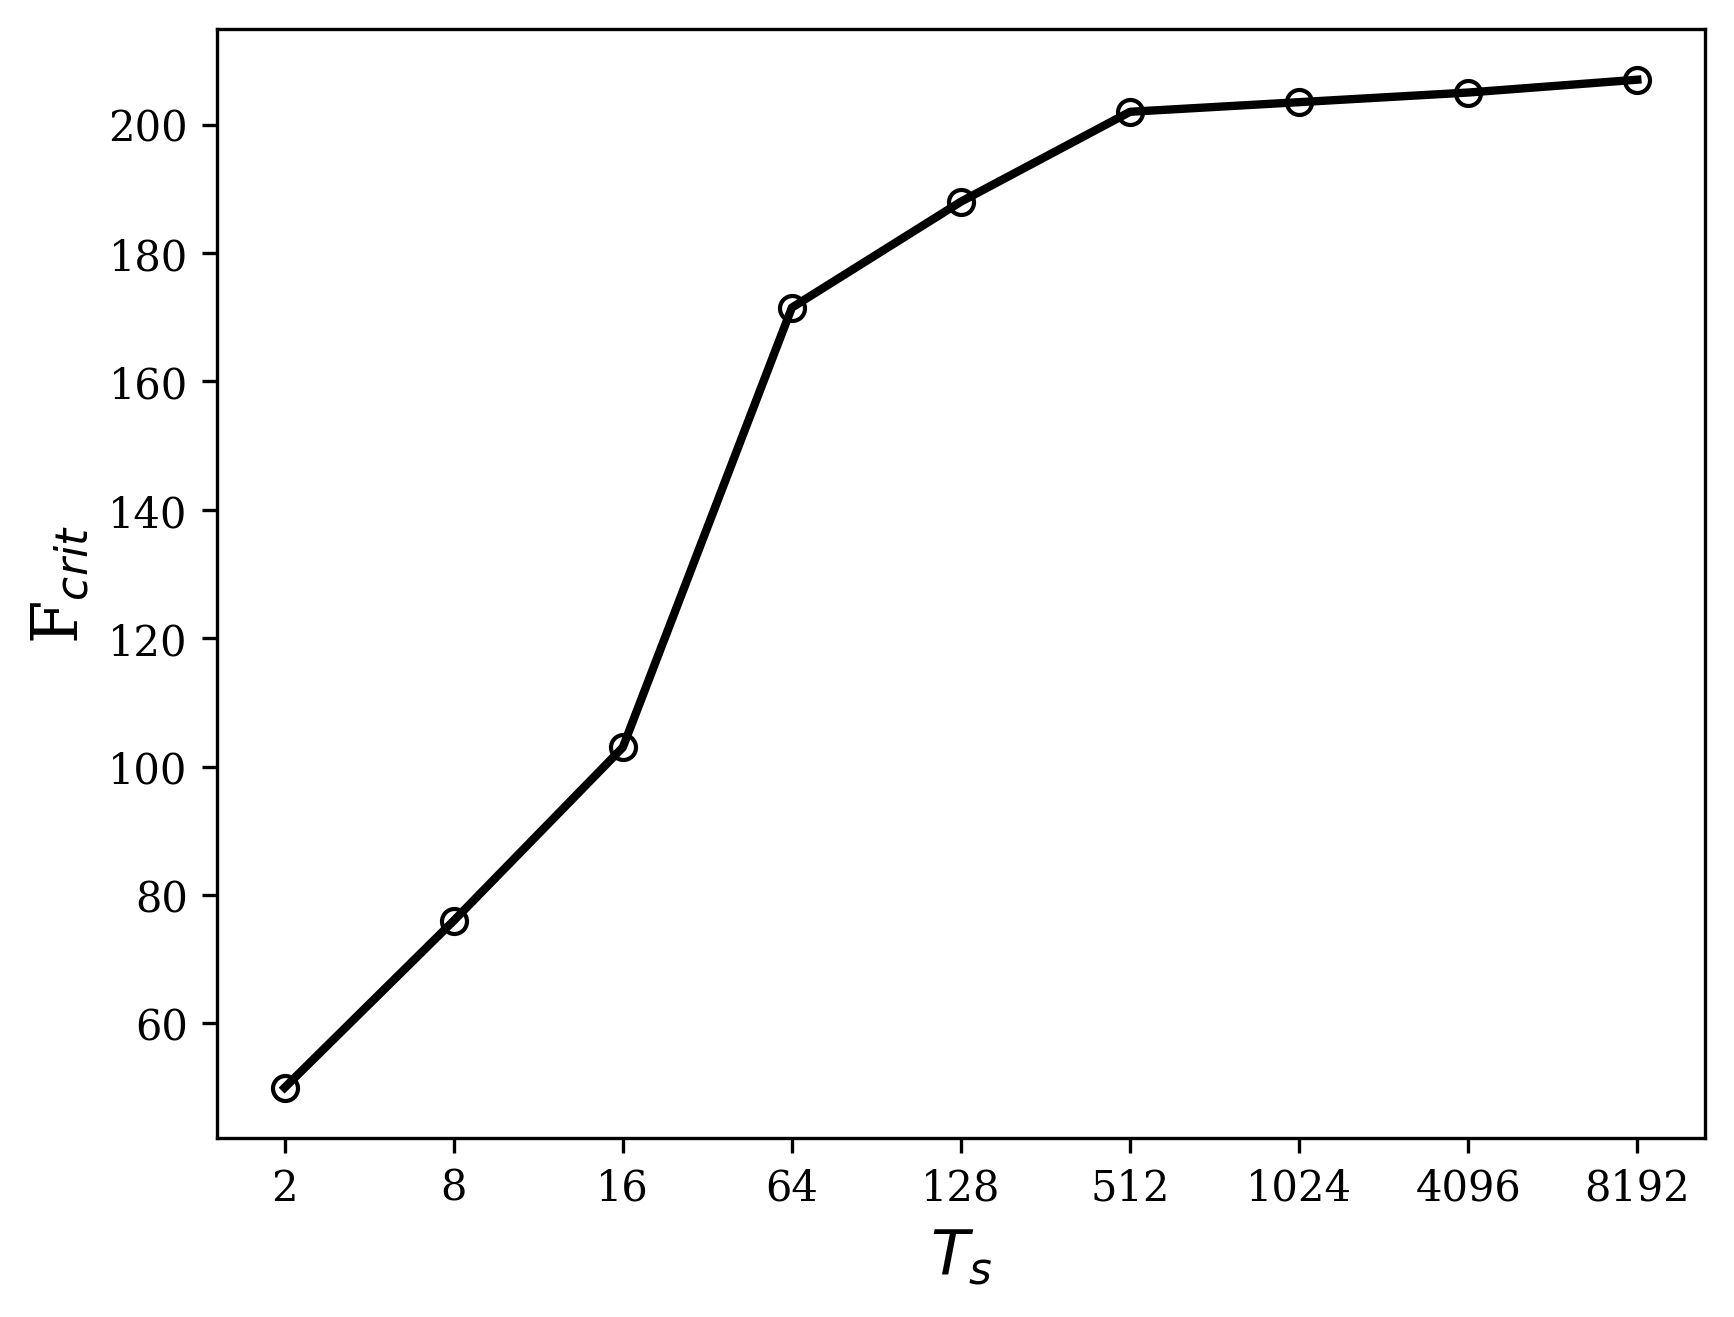
\includegraphics[width=\textwidth]{figures/force_ts.png}

    \caption{Força crítica em função do $T_{s}$. Podemos observar que a força cresce com o parâmetro $T_{s}$ até atingir um platô a partir de $T_{s} = 512$. Nessa região, a força crítica é em torno de $204.3$. Esse comportamento parece indicar, assim como para a densidade, a partir de um limite para $T_{s}$, não parece haver mais efeito do mesmo sobre as propriedades da fibrila.} 

    \label{}
\end{figure}

\begin{figure}[H]
    \centering
    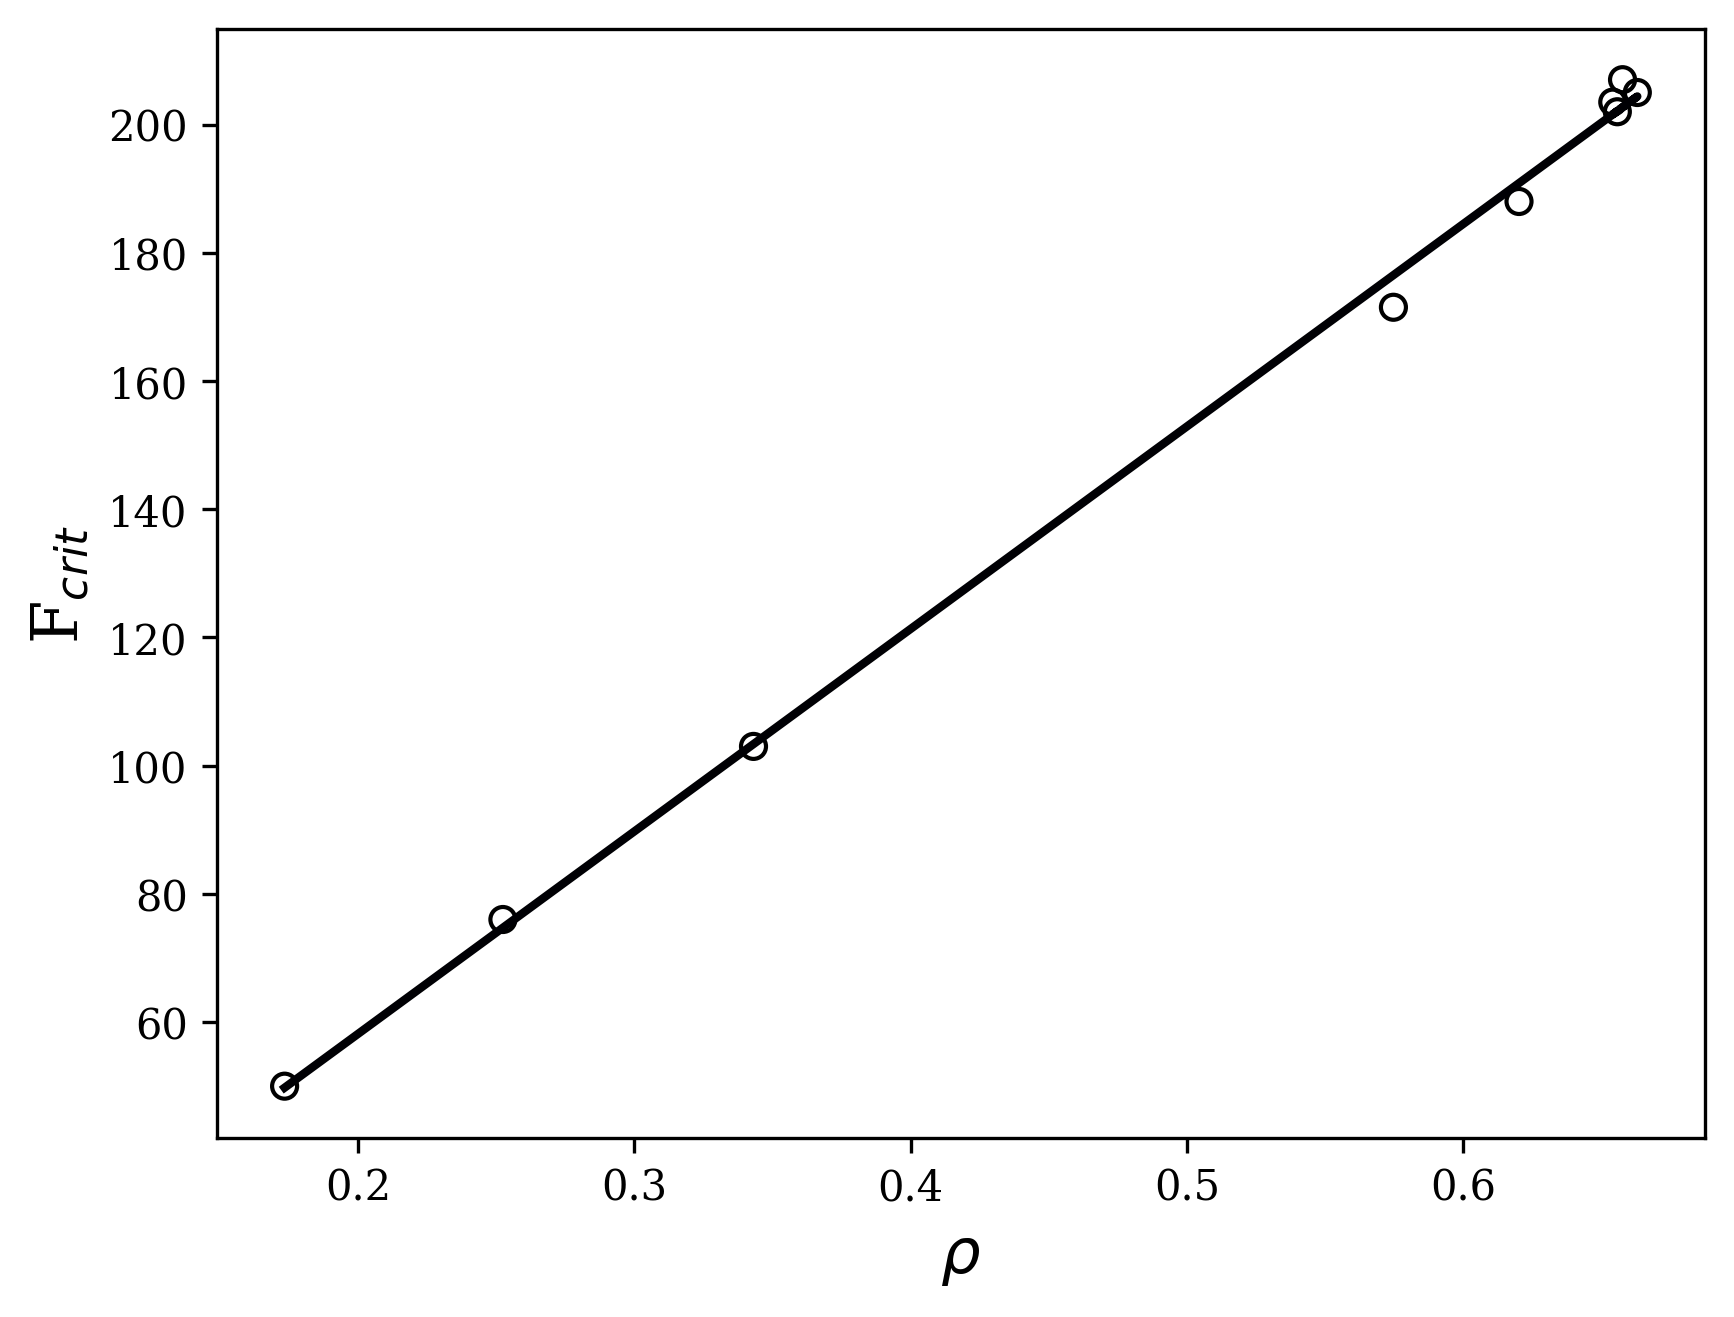
\includegraphics[width=\textwidth]{figures/force_dens.png}

    \caption{A densidade e a força crítica, em função do $T_{s}$ são curvas de comportamento bastante similares, o que nos leva a questionar como um parâmetro afeta o outro. Tomando a força em função da densidade, observamos um inesperado comportamento linear, de modo que $\alpha = 315.87$. Ao se aproximar da densidade máxima, vemos que a força aparece toda em uma região muito próxima, evocando o platô que observamos anteriormente.} 

    \label{}
\end{figure}

\begin{figure}[H]
    \centering
    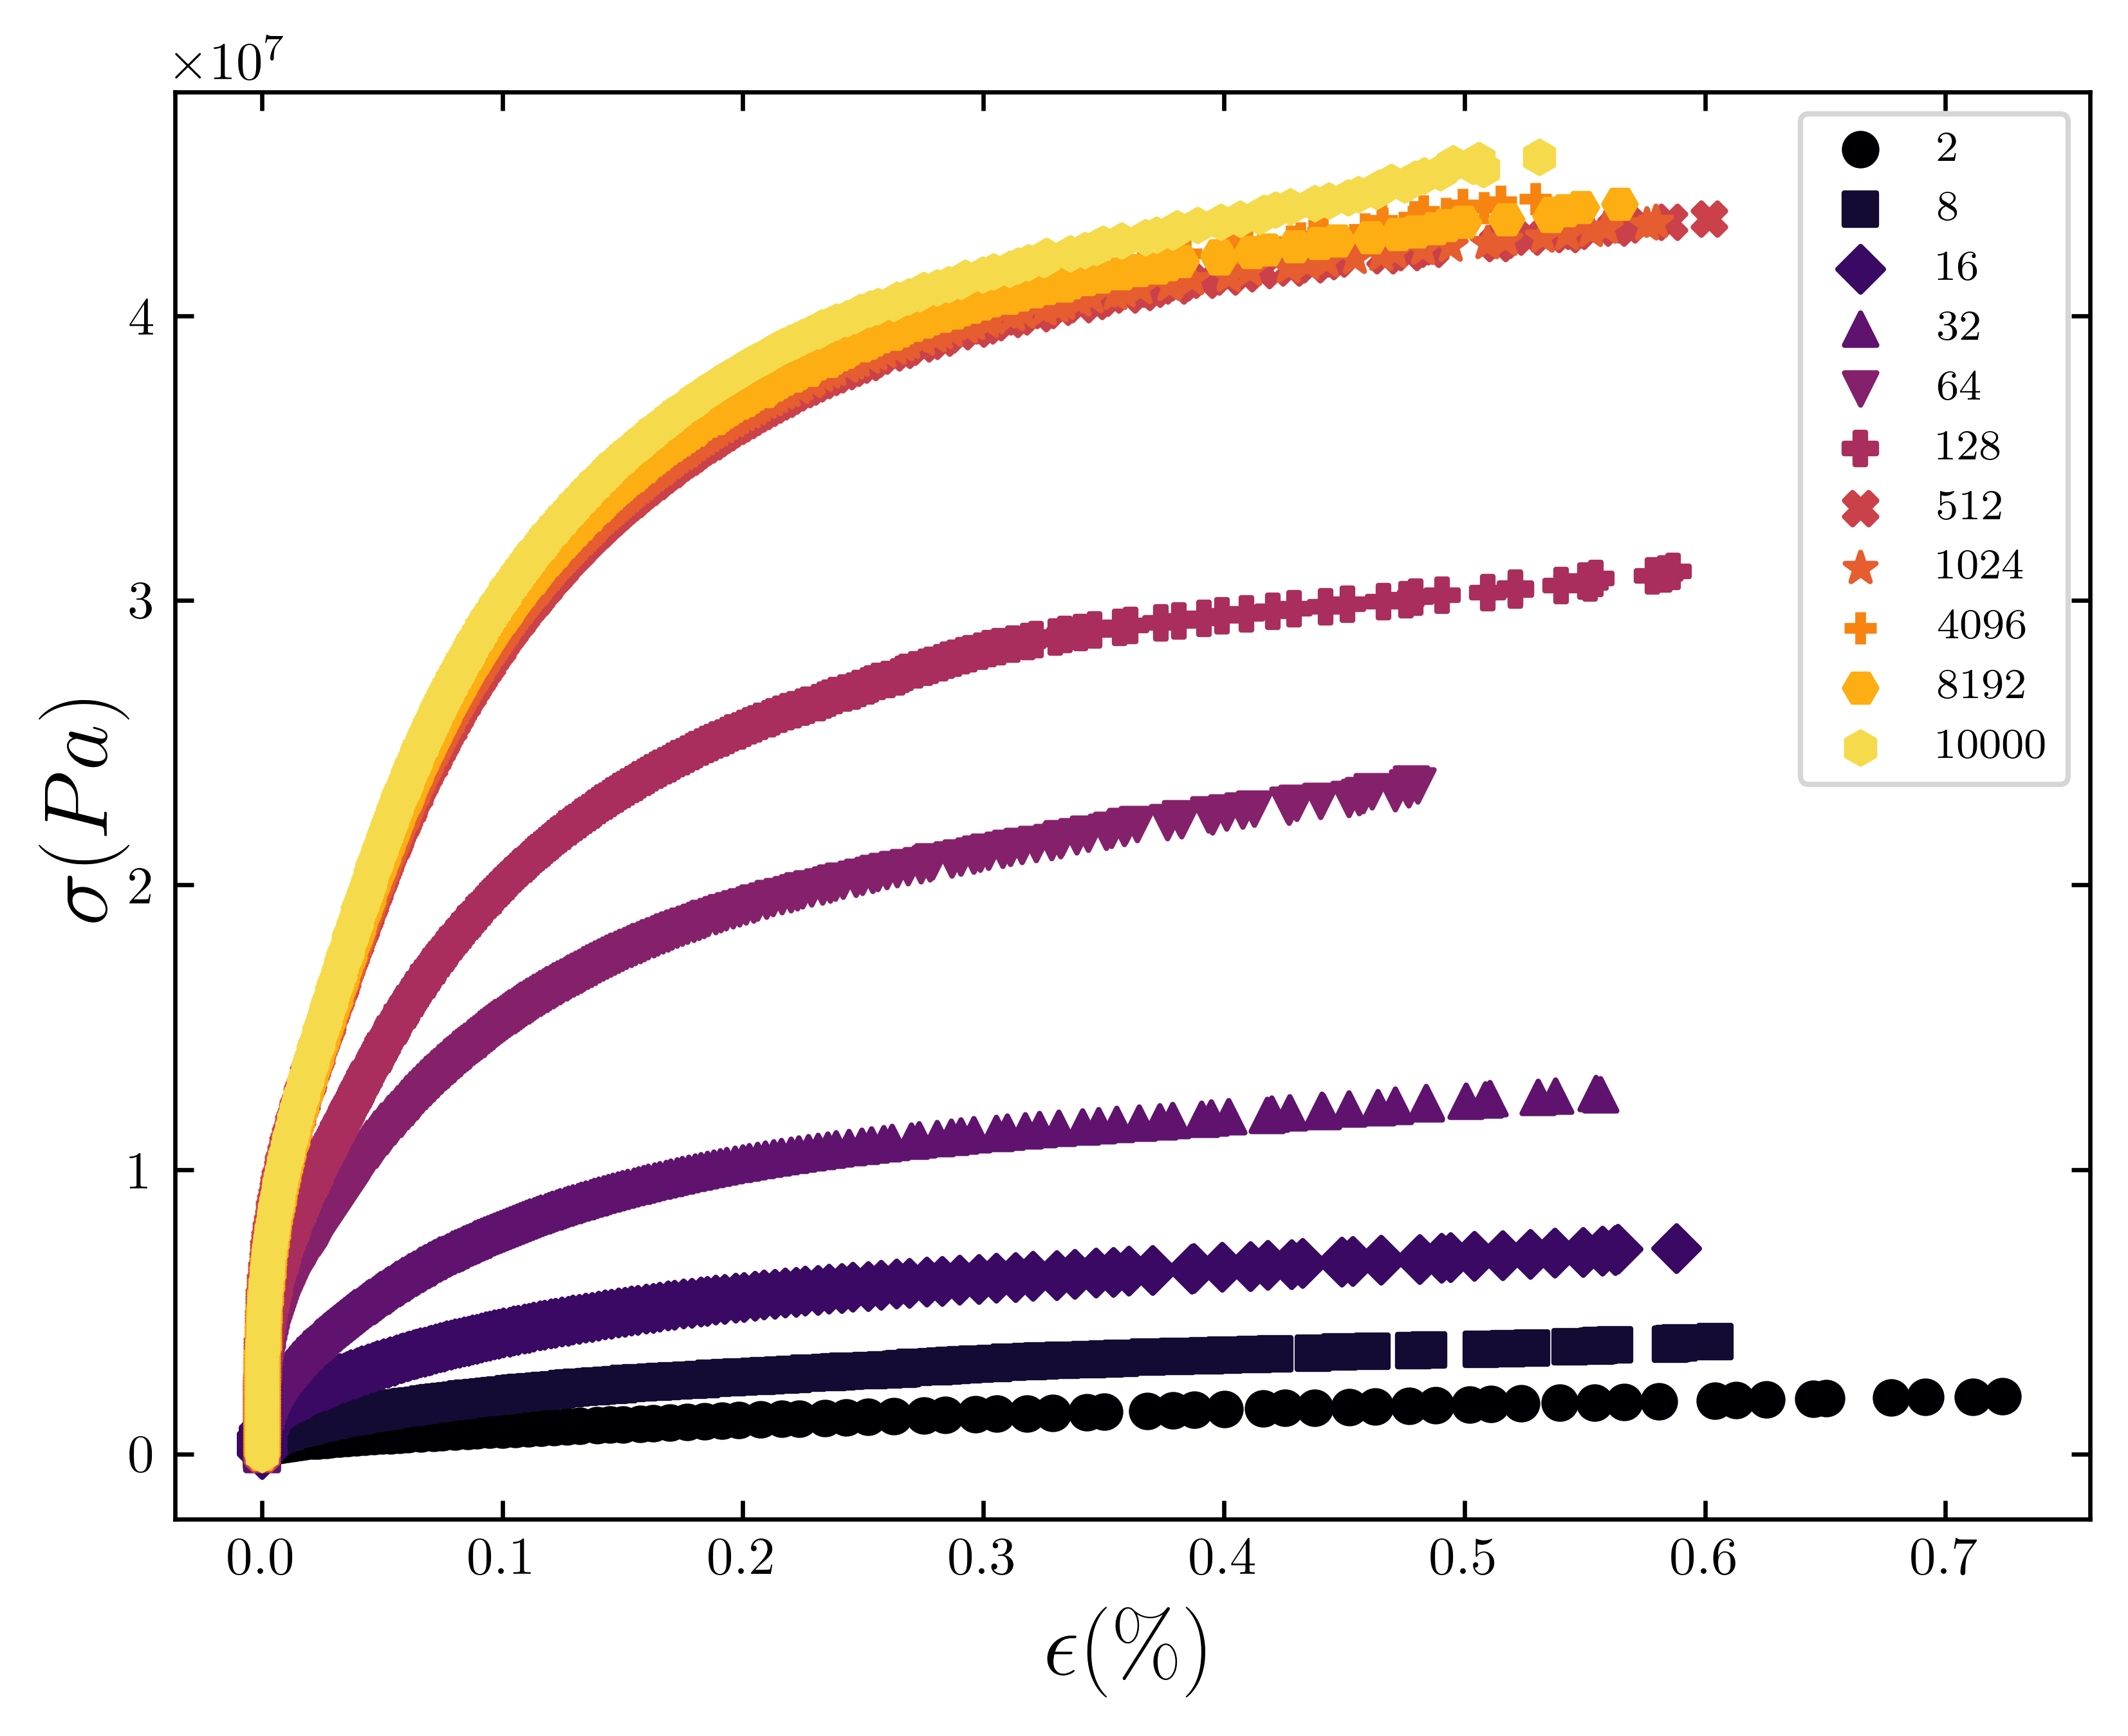
\includegraphics[width=\textwidth]{figures/stress_strain.png}

    \caption{Para analisar o efeito da força sobre as fibrilas, construímos a curva de Stres-Strain para cada valor do parâmetro $T_{s}$. Podemos ver que o aumento desse parâmetro implica no aumento da deformação suportada pela fibrila. Além disso, observamos que para os valores de $T_{s}>=512$, o comportamento das fibrilas é basicamente o mesmo com relação a deformação. Isso é um indício que podemos obter uma estrutura resistente sem um grande custo de $T_{s}$.}

    \label{}
\end{figure}

\begin{figure}[H]
    \centering
    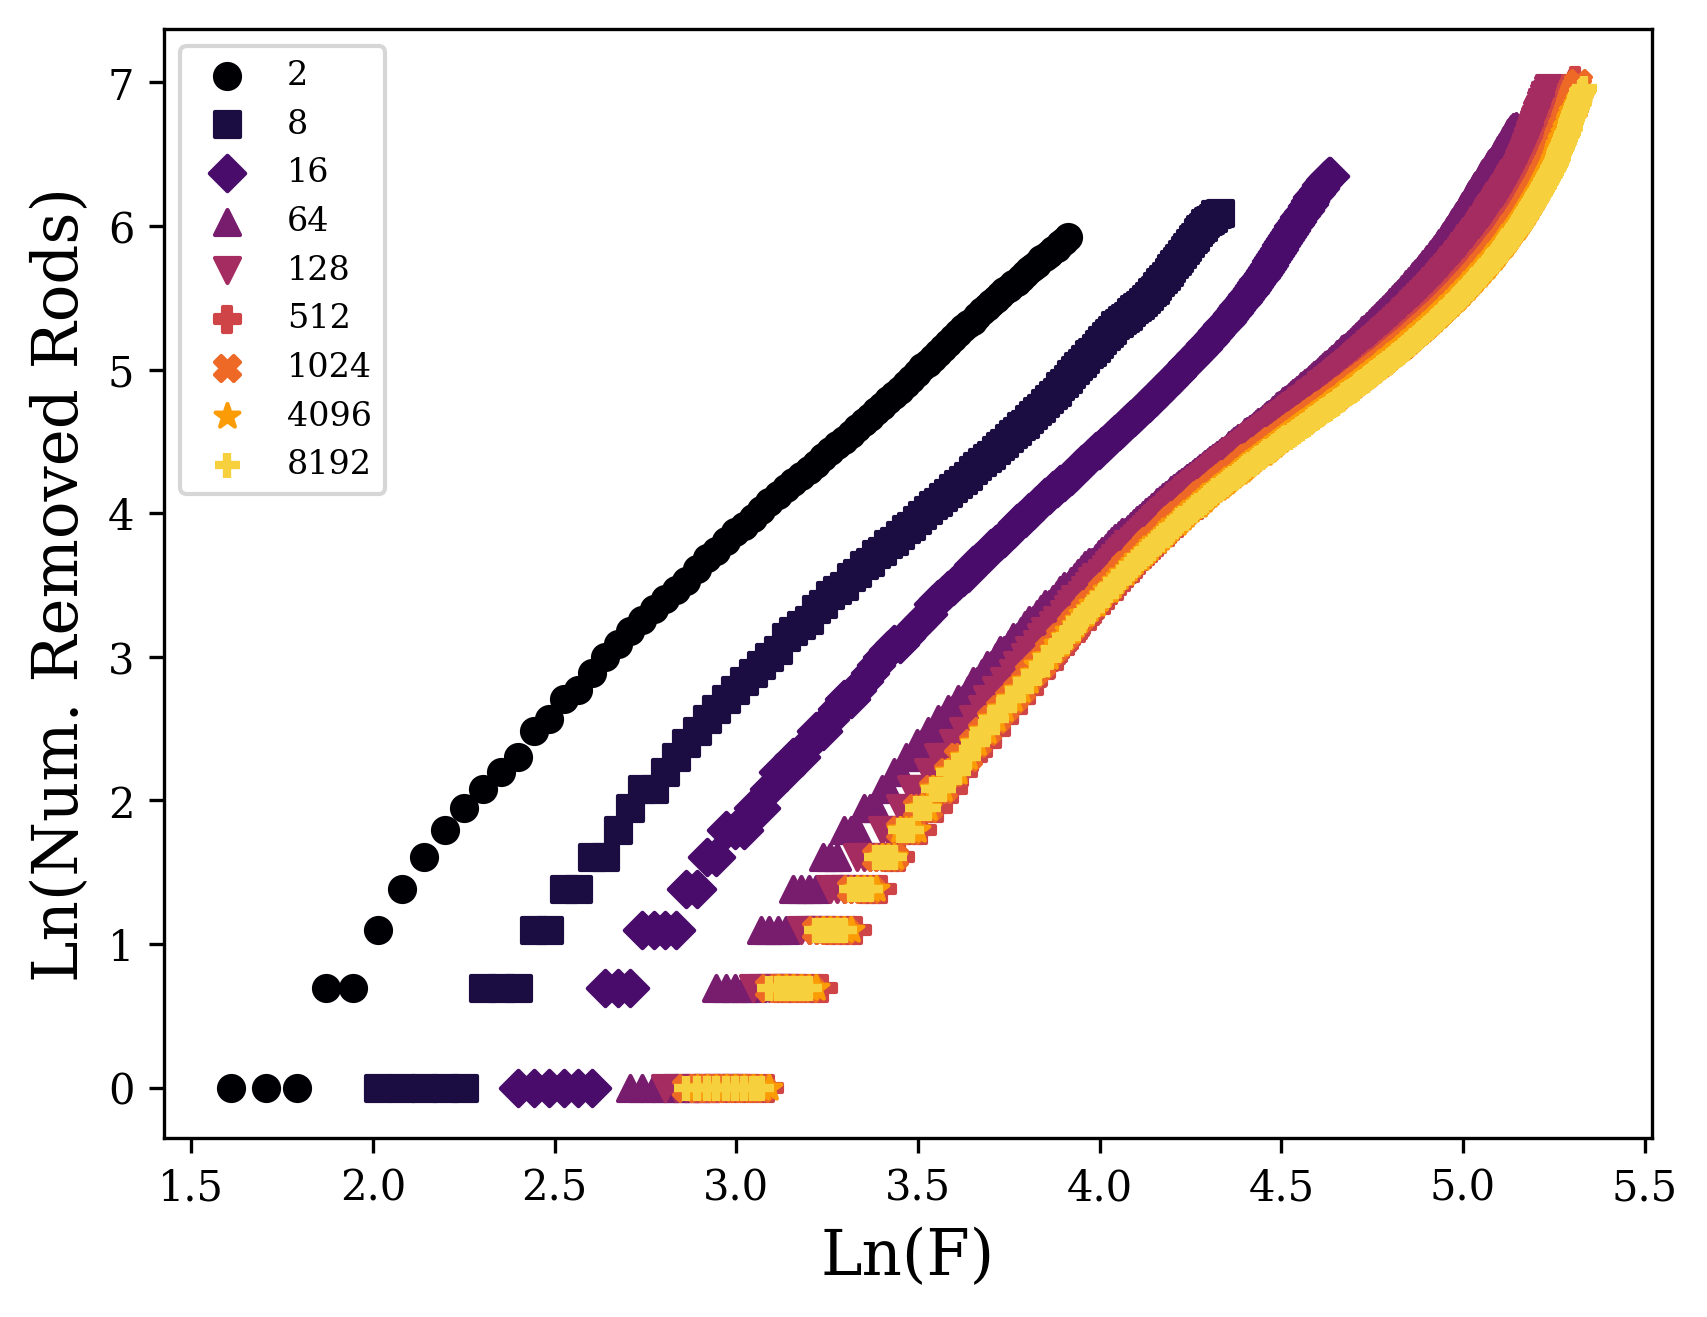
\includegraphics[width=\textwidth]{figures/ln_stress_strain.png}

    \caption{Ao analisarmos a curva de Stress-Strain em escala log natural, observamos que as curvas se tornaram praticamente paralelas. Fazendo regressão, observamos que os coeficientes angulares são bastante próximo. As curvas não se sobrepõem por causa do coeficiente linear, que nesse caso, é simplesmente o $Ln(F)$ mínimo para começar a causar quebras na fibrila, algo semelhante a função trabalho no efeito fotoelétrico. Para o parâmetro $T_{s}$ baixo, temos que o comportamento linear percorre toda a curva, contudo, podemos observar que a esse parâmetro aumenta, um comportamento não linear começa a surgir na região final da curva. Esse comportamento deve ser devido a região de deformação elástica da fibrila, de forma que conseguimos determinar melhor essa região pela análise da sua curva em escala log normal.} 

    \label{}
\end{figure}

\bibliographystyle{plain} % Set the bibliography style
\bibliography{ref} % Include your .bib file (without the .bib extension)


    
\end{document}
